\chapter{矢量与旋量的几何}

如果我们将一个闵氏空间的矢量$\boldsymbol{v}$在自然基底$(e_{t} ,e_{x} ,e_{y} ,e_{z} )$下展开得到分量$( t,x,y,z)$,其内积为$v^{2} =t^{2} -x^{2} -y^{2} -z^{2}$。但如果我们换一组类光基底展开:
\begin{equation*}
	\begin{aligned}
		\boldsymbol{v} & =te_{t} +xe_{x} +ye_{y} +ze_{z}\\
		& =\left(\frac{t+z}{\sqrt{2}}\right)\boldsymbol{l} +\left(\frac{t-z}{\sqrt{2}}\right)\boldsymbol{n} +\left(\frac{x+\mathrm{i} y}{\sqrt{2}}\right)\boldsymbol{m} +\left(\frac{x-\mathrm{i} y}{\sqrt{2}}\right)\overline{\boldsymbol{m}} ,
	\end{aligned}
\end{equation*}
其中
\begin{equation*}
	\boldsymbol{l} \equiv \frac{e_{t} +e_{z}}{\sqrt{2}} ,\quad \boldsymbol{n} \equiv \frac{e_{t} -e_{z}}{\sqrt{2}} ,\quad \boldsymbol{m} \equiv \frac{e_{x} -\mathrm{i} e_{y}}{\sqrt{2}} ,\quad \overline{\boldsymbol{m}} \equiv \frac{e_{x} +\mathrm{i} e_{y}}{\sqrt{2}}
\end{equation*}
这样我们就能将$\boldsymbol{v}$写成一个厄米矩阵:
\begin{equation*}
	v\rightarrow \frac{1}{\sqrt{2}}\begin{pmatrix}
		t+z & x+\mathrm{i} y\\
		x-\mathrm{i} y & t-z
	\end{pmatrix} .
\end{equation*}
如果$v$是类光矢量,那么我们自然有$\det\boldsymbol{v} =(t^{2} -x^{2} -y^{2} -z^{2} )/2=0$,这意味着其秩不超过$1$,可以用两个复向量构建:
\begin{equation*}
	\frac{1}{\sqrt{2}}\begin{pmatrix}
		t+z & x+\mathrm{i} y\\
		x-\mathrm{i} y & t-z
	\end{pmatrix} =\alpha \alpha ^{\dagger } ,\alpha =\begin{pmatrix}
		\xi \\
		\eta 
	\end{pmatrix}
\end{equation*}
我们称$\alpha $为\textbf{旋量}。实际上,对于一个非类光矢量我们也能定义对应的旋量的概念。通过考虑在旋量上的作用,我们也能清晰地了解洛伦兹群的结构。除此之外,类光矢量决定了时空的因果结构,而这也与旋量密切相关。一个时空是否存在旋量结构与其\textbf{整体拓扑}有关,而Geroch证明了\parencite{geroch1968spinor},一个非紧的时空存在旋量结构,当且仅当它存在连续的正交归一的闵氏标架场。因此,从旋量出发构建矢量,以及相对论理论则是更基本的也是更容易的。

\section{闵氏向量空间}

闵氏向量空间是所谓\textbf{世界矢量}(world vector)的空间,其由狭义相对论时空中的位置矢量的集合构成。在弯曲时空中,闵氏向量空间作为时空点的切空间出现。它是$\mathbb{R}$上带有定向的实向量空间$\mathbb{V}$,带有双线性的内积$( +,-,-,-)$。$\mathbb{V}$配备了一个自然基$\boldsymbol{t} ,\boldsymbol{x} ,\boldsymbol{y} ,\boldsymbol{z}$,即任何一个矢量都可以用这组基展开:
\begin{equation*}
	\boldsymbol{U} =U^{0}\boldsymbol{t} +U^{1}\boldsymbol{x} +U^{2}\boldsymbol{y} +U^{3}\boldsymbol{z} ,\quad U^{i} \in \mathbb{R} .
\end{equation*}
我们称$\mathbb{V}$中的一组基为\textbf{标架}(tetrad),表示为$\boldsymbol{g}_{i}$,例如标架$(\boldsymbol{t} ,\boldsymbol{x} ,\boldsymbol{y} ,\boldsymbol{z})$可以表示为
\begin{equation*}
	\boldsymbol{t} =\boldsymbol{g}_{0} ,\quad \boldsymbol{x} =\boldsymbol{g}_{1} ,\quad \boldsymbol{y} =\boldsymbol{g}_{2} ,\quad \boldsymbol{z} =\boldsymbol{g}_{3} ,
\end{equation*}
那么一个矢量就可以表示为$\boldsymbol{U} =U^{i}\boldsymbol{g}_{i}$。如果我们考虑另一组标架$\boldsymbol{g}_{\tilde{\imath }}$,我们知道
\begin{equation*}
	\boldsymbol{g}_{i} =g{_{i}}^{\tilde{0}}\boldsymbol{g}_{\tilde{0}} +g{_{i}}^{\tilde{1}}\boldsymbol{g}_{\tilde{1}} +g{_{i}}^{\tilde{2}}\boldsymbol{g}_{\tilde{2}} +g{_{i}}^{\tilde{3}}\boldsymbol{g}_{\tilde{3}} =g{_{i}}^{\tilde{\jmath }}\boldsymbol{g}_{\hat{\jmath }} .
\end{equation*}
矩阵$g{_{i}}^{\tilde{\jmath }}$构成了一个非奇异矩阵,如果其行列式是正的,我们称这两个标架有相同的定向,如果是负的,我们称这两个标架有相反的定向。注意这里的定向构成了一个等价关系,因此所有标架可以归为两个等价类,我们称其中一个为正规(proper)的标架,另一个为非正规的。



度规$( +,-,-,-)$意味着我们有一个自然标架$\boldsymbol{g}_{i} =(\boldsymbol{t} ,\boldsymbol{x} ,\boldsymbol{y} ,\boldsymbol{z})$,给出
\begin{equation*}
	\eta _{ij} =\boldsymbol{g}_{i} \cdot \boldsymbol{g}_{j} =\operatorname{diag}( 1,-1,-1,-1) ,
\end{equation*}
我们称这组标架为闵氏标架。注意,二次型的惯性定理告诉我们,对于所有正交标架,自内积的正负符号是不变的。



除了一般的定义内积的方式,我们注意到内积还可以用洛伦兹范数定义:
\begin{equation*}
	\boldsymbol{U} \cdot \boldsymbol{V} =\frac{1}{2}( \| \boldsymbol{U} +\boldsymbol{V} \| -\| \boldsymbol{U} \| -\| \boldsymbol{V} \| ) ,\| \boldsymbol{U} \| \equiv \boldsymbol{U} \cdot \boldsymbol{U} .
\end{equation*}
其中我们称
\begin{equation*}
	\begin{cases}
		\begin{drcases}
			\| \boldsymbol{U} \|  >0 & \text{类时矢量}\\
			\| \boldsymbol{U} \| < 0 & \text{类空矢量}
		\end{drcases}\text{因果矢量}\\
		\| \boldsymbol{U} \| =0 \quad \text{类光矢量} .
	\end{cases}
\end{equation*}
根据Schwarz不等式,对于两个因果矢量,我们有:
\begin{equation*}
	\begin{aligned}
		|U^{0} V^{0} |\geq  & \{(U^{1} )^{2} +(U^{2} )^{2} +(U^{3} )^{2} \}^{1/2} \{(V^{1} )^{2} +(V^{2} )^{2} +(V^{3} )^{2} \}^{1/2}\\
		\geq  & U^{1} V^{1} +U^{2} V^{2} +U^{3} V^{3} ,
	\end{aligned}
\end{equation*}
我们容易看出$\boldsymbol{U} \cdot \boldsymbol{V}$的符号与$U^{0} V^{0}$一致,因此我们可以用$U^{0}$的符号来区分因果矢量,将其分为\textbf{指向未来}和\textbf{指向过去}的。如果$\boldsymbol{t}$是指向未来的类时矢量,那么我们称$(\boldsymbol{t} ,\boldsymbol{x} ,\boldsymbol{y} ,\boldsymbol{z})$为正时(orthochronous)的。



与闵氏向量空间不同的是,所谓的闵氏时空$\mathbb{M}$是一个仿射空间(affine space),即没有原点的选择,其与闵氏向量空间的关系为存在一个映射
\begin{equation*}
	\operatorname{vec:}\mathbb{M} \times \mathbb{M}\rightarrow \mathbb{V} ,
\end{equation*}
其中
\begin{equation*}
	\operatorname{vec} (P,Q)+\operatorname{vec} (Q,R)=\operatorname{vec} (P,R).
\end{equation*}
因此我们可以令$\operatorname{vec} (P,Q)\equiv \overrightarrow{PQ} \in \mathbb{V}$,而这意味着$\mathbb{V}$自然诱导出了一个范数$\upPhi $:
\begin{equation*}
	\upPhi \equiv \| \operatorname{vec} (P,Q)\| =(Q^{0} -P^{0} )^{2} -(Q^{1} -P^{1} )^{2} -(Q^{2} -P^{2} )^{2} -(Q^{3} -P^{3} )^{2} .
\end{equation*}
$\mathbb{V}$上的线性保范数自变换被称为\textbf{洛伦兹变换}。如果与此同时保定向和时间定向,那么称其为限制性洛伦兹变换,而$\mathbb{M}$上的线性保范数$\upPhi $的变换被称为庞加莱变换,这样的变换在$\mathbb{V}$上自动诱导出了洛伦兹变换。

\section{类光矢量与自旋变换}

对于一个限制性的闵氏标架$(\boldsymbol{t} ,\boldsymbol{x} ,\boldsymbol{y} ,\boldsymbol{z})$,我们记其展开系数为
\begin{equation*}
	\boldsymbol{U} =T\boldsymbol{t} +X\boldsymbol{x} +Y\boldsymbol{y} +Z\boldsymbol{z} .
\end{equation*}
如果$\boldsymbol{U}$是类光的,那么我们知道
\begin{equation}
	T^{2} -X^{2} -Y^{2} -Z^{2} =0,
	\label{eq:lightlike vector}
\end{equation}
这自然构成了一个三维的双曲面,如图\ref{fig:lightcone}所示。

\begin{figure}[h]
	\centering
	% Gradient Info

\tikzset {_ahkgnj71m/.code = {\pgfsetadditionalshadetransform{ \pgftransformshift{\pgfpoint{262.5 bp } { 228 bp }  }  \pgftransformscale{3 }  }}}
\pgfdeclareradialshading{_bn94sccyc}{\pgfpoint{-88bp}{-56bp}}{rgb(0bp)=(0.96,0.96,0.96);
	rgb(0bp)=(0.96,0.96,0.96);
	rgb(5.25bp)=(0.86,0.86,0.89);
	rgb(12.25bp)=(0.72,0.73,0.78);
	rgb(20bp)=(0.87,0.87,0.89);
	rgb(25bp)=(0.96,0.96,0.96);
	rgb(400bp)=(0.96,0.96,0.96)}

% Gradient Info

\tikzset {_8s0cjt0cb/.code = {\pgfsetadditionalshadetransform{ \pgftransformshift{\pgfpoint{-69 bp } { 489 bp }  }  \pgftransformscale{3 }  }}}
\pgfdeclareradialshading{_arll6v0fl}{\pgfpoint{24bp}{-192bp}}{rgb(0bp)=(0.96,0.96,0.96);
	rgb(0bp)=(0.96,0.96,0.96);
	rgb(5.25bp)=(0.86,0.86,0.89);
	rgb(12.25bp)=(0.72,0.73,0.78);
	rgb(20bp)=(0.87,0.87,0.89);
	rgb(25bp)=(0.96,0.96,0.96);
	rgb(400bp)=(0.96,0.96,0.96)}

% Gradient Info

\tikzset {_xb2d8cp10/.code = {\pgfsetadditionalshadetransform{ \pgftransformshift{\pgfpoint{0 bp } { 0 bp }  }  \pgftransformrotate{0 }  \pgftransformscale{2 }  }}}
\pgfdeclarehorizontalshading{_9gf5dp3f7}{150bp}{rgb(0bp)=(0.6,0.85,1);
	rgb(37.5bp)=(0.6,0.85,1);
	rgb(62.5bp)=(0,0.5,0.5);
	rgb(100bp)=(0,0.5,0.5)}

% Gradient Info

\tikzset {_jwa1tz4np/.code = {\pgfsetadditionalshadetransform{ \pgftransformshift{\pgfpoint{0 bp } { 0 bp }  }  \pgftransformrotate{0 }  \pgftransformscale{2 }  }}}
\pgfdeclarehorizontalshading{_k1lfmkpnc}{150bp}{rgb(0bp)=(0.6,0.85,1);
	rgb(37.5bp)=(0.6,0.85,1);
	rgb(62.5bp)=(0,0.5,0.5);
	rgb(100bp)=(0,0.5,0.5)}

% Gradient Info

\tikzset {_lmp8db242/.code = {\pgfsetadditionalshadetransform{ \pgftransformshift{\pgfpoint{0 bp } { 0 bp }  }  \pgftransformscale{1 }  }}}
\pgfdeclareradialshading{_pt7yztjpq}{\pgfpoint{0bp}{0bp}}{rgb(0bp)=(1,1,1);
	rgb(0bp)=(1,1,1);
	rgb(25bp)=(0,0,0);
	rgb(400bp)=(0,0,0)}

% Gradient Info

\tikzset {_ksf0j3lzx/.code = {\pgfsetadditionalshadetransform{ \pgftransformshift{\pgfpoint{0 bp } { 0 bp }  }  \pgftransformscale{1 }  }}}
\pgfdeclareradialshading{_sd0lfnh1v}{\pgfpoint{0bp}{0bp}}{rgb(0bp)=(1,1,1);
	rgb(0bp)=(1,1,1);
	rgb(25bp)=(0,0,0);
	rgb(400bp)=(0,0,0)}

% Gradient Info

\tikzset {_sfydnlf8x/.code = {\pgfsetadditionalshadetransform{ \pgftransformshift{\pgfpoint{-246 bp } { -414 bp }  }  \pgftransformscale{2 }  }}}
\pgfdeclareradialshading{_xedxn5b0y}{\pgfpoint{136bp}{224bp}}{rgb(0bp)=(0.96,0.96,0.96);
	rgb(0bp)=(0.96,0.96,0.96);
	rgb(5.25bp)=(0.86,0.86,0.89);
	rgb(12.25bp)=(0.72,0.73,0.78);
	rgb(20bp)=(0.87,0.87,0.89);
	rgb(25bp)=(0.96,0.96,0.96);
	rgb(400bp)=(0.96,0.96,0.96)}
\tikzset{every picture/.style={line width=0.75pt}} %set default line width to 0.75pt   

\begin{tikzpicture}[x=0.75pt,y=0.75pt,yscale=-1,xscale=1]
%uncomment if require: \path (0,240); %set diagram left start at 0, and has height of 240

%Shape: Triangle [id:dp9971590043766994] 
\draw  [draw opacity=0][shading=_bn94sccyc,_ahkgnj71m] (316.92,132.48) -- (388.83,216.92) -- (245,216.92) -- cycle ;
%Shape: Triangle [id:dp8161858650868445] 
\draw  [draw opacity=0][shading=_arll6v0fl,_8s0cjt0cb] (316.92,132.48) -- (388.83,48.85) -- (245,48.85) -- cycle ;
%Shape: Trapezoid [id:dp9657525832586118] 
\draw  [dash pattern={on 4.5pt off 4.5pt}] (242.44,151.83) -- (249.4,114.75) -- (384.44,114.75) -- (391.4,151.83) -- cycle ;
%Shape: Ellipse [id:dp6991681555350466] 
\draw  [fill={rgb, 255:red, 255; green, 255; blue, 255 }  ,fill opacity=1 ][dash pattern={on 0.84pt off 2.51pt}][line width=0.75]  (245,48.85) .. controls (245,38.22) and (277.2,29.6) .. (316.92,29.6) .. controls (356.64,29.6) and (388.83,38.22) .. (388.83,48.85) .. controls (388.83,59.49) and (356.64,68.1) .. (316.92,68.1) .. controls (277.2,68.1) and (245,59.49) .. (245,48.85) -- cycle ;
%Straight Lines [id:da6048999871668166] 
\draw    (316.92,49.67) -- (316.92,216.92) ;
%Straight Lines [id:da8004605643454383] 
\draw [shading=_9gf5dp3f7,_xb2d8cp10]   (316.92,133.29) -- (245,49.67) ;
%Straight Lines [id:da5641309946559745] 
\draw [shading=_k1lfmkpnc,_jwa1tz4np]   (316.92,133.29) -- (388.83,49.67) ;
\draw [shift={(316.92,133.29)}, rotate = 310.7] [color={rgb, 255:red, 0; green, 0; blue, 0 }  ][fill={rgb, 255:red, 0; green, 0; blue, 0 }  ][line width=0.75]      (0, 0) circle [x radius= 3.35, y radius= 3.35]   ;
%Shape: Ellipse [id:dp5518313431037392] 
\draw  [fill={rgb, 255:red, 255; green, 255; blue, 255 }  ,fill opacity=1 ][dash pattern={on 0.84pt off 2.51pt}] (245,216.92) .. controls (245,206.29) and (277.2,197.67) .. (316.92,197.67) .. controls (356.64,197.67) and (388.83,206.29) .. (388.83,216.92) .. controls (388.83,227.55) and (356.64,236.17) .. (316.92,236.17) .. controls (277.2,236.17) and (245,227.55) .. (245,216.92) -- cycle ;
%Straight Lines [id:da7941441583124655] 
\draw [shading=_pt7yztjpq,_lmp8db242]   (316.92,133.29) -- (245,216.92) ;
%Straight Lines [id:da3585204572517584] 
\draw [shading=_sd0lfnh1v,_ksf0j3lzx]   (316.92,133.29) -- (388.83,216.92) ;

%Straight Lines [id:da5552987525760773] 
\draw    (316.92,133.29) -- (316.92,4.92) ;
\draw [shift={(316.92,2.92)}, rotate = 90] [color={rgb, 255:red, 0; green, 0; blue, 0 }  ][line width=0.75]    (10.93,-3.29) .. controls (6.95,-1.4) and (3.31,-0.3) .. (0,0) .. controls (3.31,0.3) and (6.95,1.4) .. (10.93,3.29)   ;
%Shape: Trapezoid [id:dp11767877524393056] 
\draw  [dash pattern={on 4.5pt off 4.5pt}] (242.44,105.83) -- (249.4,68.75) -- (384.44,68.75) -- (391.4,105.83) -- cycle ;
%Shape: Ellipse [id:dp5991835638059029] 
\draw  [dash pattern={on 0.84pt off 2.51pt}] (275.82,83.92) .. controls (275.82,77.84) and (294.22,72.92) .. (316.92,72.92) .. controls (339.61,72.92) and (358.01,77.84) .. (358.01,83.92) .. controls (358.01,89.99) and (339.61,94.92) .. (316.92,94.92) .. controls (294.22,94.92) and (275.82,89.99) .. (275.82,83.92) -- cycle ;
%Shape: Trapezoid [id:dp03040677334653208] 
\draw  [dash pattern={on 4.5pt off 4.5pt}] (242.44,204.83) -- (249.4,167.75) -- (384.44,167.75) -- (391.4,204.83) -- cycle ;
%Shape: Ellipse [id:dp16350683172549307] 
\draw  [dash pattern={on 0.84pt off 2.51pt}] (275.82,182.92) .. controls (275.82,176.84) and (294.22,171.92) .. (316.92,171.92) .. controls (339.61,171.92) and (358.01,176.84) .. (358.01,182.92) .. controls (358.01,188.99) and (339.61,193.92) .. (316.92,193.92) .. controls (294.22,193.92) and (275.82,188.99) .. (275.82,182.92) -- cycle ;
%Curve Lines [id:da5556333810941549] 
\draw    (135,132.5) .. controls (142.75,93.31) and (217.32,126.24) .. (270.24,90.04) ;
\draw [shift={(271.83,88.92)}, rotate = 144.36] [color={rgb, 255:red, 0; green, 0; blue, 0 }  ][line width=0.75]    (10.93,-3.29) .. controls (6.95,-1.4) and (3.31,-0.3) .. (0,0) .. controls (3.31,0.3) and (6.95,1.4) .. (10.93,3.29)   ;
%Curve Lines [id:da7958034781622496] 
\draw    (135,164.5) .. controls (141.76,204.51) and (240.81,150.03) .. (274.81,181.92) ;
\draw [shift={(275.82,182.92)}, rotate = 225.86] [color={rgb, 255:red, 0; green, 0; blue, 0 }  ][line width=0.75]    (10.93,-3.29) .. controls (6.95,-1.4) and (3.31,-0.3) .. (0,0) .. controls (3.31,0.3) and (6.95,1.4) .. (10.93,3.29)   ;
%Shape: Circle [id:dp0994570688091998] 
\path  [shading=_xedxn5b0y,_sfydnlf8x] (514.58,116.21) .. controls (514.58,97.59) and (529.68,82.5) .. (548.29,82.5) .. controls (566.91,82.5) and (582,97.59) .. (582,116.21) .. controls (582,134.82) and (566.91,149.92) .. (548.29,149.92) .. controls (529.68,149.92) and (514.58,134.82) .. (514.58,116.21) -- cycle ; % for fading 
\draw   (514.58,116.21) .. controls (514.58,97.59) and (529.68,82.5) .. (548.29,82.5) .. controls (566.91,82.5) and (582,97.59) .. (582,116.21) .. controls (582,134.82) and (566.91,149.92) .. (548.29,149.92) .. controls (529.68,149.92) and (514.58,134.82) .. (514.58,116.21) -- cycle ; % for border 

%Curve Lines [id:da472614963631488] 
\draw    (358.01,83.92) .. controls (365.77,44.73) and (463.84,49.81) .. (516.26,84.85) ;
\draw [shift={(517.83,85.92)}, rotate = 214.7] [color={rgb, 255:red, 0; green, 0; blue, 0 }  ][line width=0.75]    (10.93,-3.29) .. controls (6.95,-1.4) and (3.31,-0.3) .. (0,0) .. controls (3.31,0.3) and (6.95,1.4) .. (10.93,3.29)   ;
%Curve Lines [id:da301798245305416] 
\draw    (358.01,182.92) .. controls (364.78,222.93) and (504.01,203.32) .. (519.4,145.68) ;
\draw [shift={(519.83,143.92)}, rotate = 102.43] [color={rgb, 255:red, 0; green, 0; blue, 0 }  ][line width=0.75]    (10.93,-3.29) .. controls (6.95,-1.4) and (3.31,-0.3) .. (0,0) .. controls (3.31,0.3) and (6.95,1.4) .. (10.93,3.29)   ;


% Text Node
\draw (328,1.5) node [anchor=north west][inner sep=0.75pt]    {$t$};
% Text Node
\draw (396,78.5) node [anchor=north west][inner sep=0.75pt]    {$T=1$};
% Text Node
\draw (396,124.5) node [anchor=north west][inner sep=0.75pt]    {$T=0$};
% Text Node
\draw (395,172.5) node [anchor=north west][inner sep=0.75pt]    {$T=-1$};
% Text Node
\draw (78,138.5) node [anchor=north west][inner sep=0.75pt]    {$x^{2} +y^{2} +z^{2} =1$};
% Text Node
\draw (324,125.5) node [anchor=north west][inner sep=0.75pt]    {$O$};
% Text Node
\draw (370,4.5) node [anchor=north west][inner sep=0.75pt]   [align=left] {null cone};
% Text Node
\draw (361,80.5) node [anchor=north west][inner sep=0.75pt]  [font=\footnotesize]  {$S^{+}$};
% Text Node
\draw (363,173.5) node [anchor=north west][inner sep=0.75pt]  [font=\footnotesize]  {$S^{-}$};
% Text Node
\draw (329,31.5) node [anchor=north west][inner sep=0.75pt]  [font=\small]  {$\mathcal{S}^{+}$};
% Text Node
\draw (327,219.5) node [anchor=north west][inner sep=0.75pt]  [font=\small]  {$\mathcal{S}^{-}$};
% Text Node
\draw (490,106.5) node [anchor=north west][inner sep=0.75pt]    {$S^{\pm }$};

\end{tikzpicture}
	\caption{四维时空中,方程$T^{2} -X^{2} -Y^{2} -Z^{2} =0$构成的超曲面,即光锥。对于不同的$t=T$的平面在曲面上的截面构成一个二维球面,即天球。}
	\label{fig:lightcone}
\end{figure}

我们记这些指向未来(过去)的类光矢量的空间为$\mathcal{S}^{+} /\mathcal{S}^{-}$,而它们在超平面$T=1/-1$上的投影被称为$S^{+} /S^{-}$,其方程为
\begin{equation*}
	x^{2} +y^{2} +z^{2} =1.
\end{equation*}
$S^{+} /S^{-}$的内部代表了指向未来/过去的方向的集合,而其外部则是类空的方向。



现在我们回到物理,考虑一个时空中的观测者位于事件$O$处。到达其眼中的光线为穿过$O$的类光线,也就是图\ref{fig:lightcone}所示的超平面$\mathcal{S}^{-}$,如果我们考虑一个固定时刻$T$,那么这就是球面$S^{-}$。因此我们称$S^{-}$(或$\mathcal{S}^{-}$)为事件$O$的天球(celestial sphere),而称将所有源于$O$点的类光方向映射到$S^{-}$的映射称为天空映射(sky mapping)。而对于$S^{+}$我们称其为反天空映射(anti-sky mapping)。



我们可以很自然地将$S^{+} /S^{-}$看成Argand平面上的黎曼球面,而一个$\mathbb{V}$上额限制性洛伦兹变换可以被它对黎曼面的作用而唯一决定。我们可以用将$S^{+}$上的坐标$x,y,z$用球极投影(stereographic)映射到一个Argand平面的复数上。

\begin{figure}[h]
	\centering
	

% Gradient Info

\tikzset {_2zcujs10x/.code = {\pgfsetadditionalshadetransform{ \pgftransformshift{\pgfpoint{228 bp } { -600 bp }  }  \pgftransformscale{3 }  }}}
\pgfdeclareradialshading{_gt23p819p}{\pgfpoint{-80bp}{232bp}}{rgb(0bp)=(0.96,0.96,0.96);
	rgb(0bp)=(0.96,0.96,0.96);
	rgb(5.25bp)=(0.86,0.86,0.89);
	rgb(12.25bp)=(0.72,0.73,0.78);
	rgb(20bp)=(0.87,0.87,0.89);
	rgb(25bp)=(0.96,0.96,0.96);
	rgb(400bp)=(0.96,0.96,0.96)}

% Gradient Info

\tikzset {_ke7fkjhbt/.code = {\pgfsetadditionalshadetransform{ \pgftransformshift{\pgfpoint{0 bp } { 0 bp }  }  \pgftransformrotate{0 }  \pgftransformscale{2 }  }}}
\pgfdeclarehorizontalshading{_zhaeh0lf2}{150bp}{rgb(0bp)=(1,1,1);
	rgb(61.622025626046316bp)=(1,1,1);
	rgb(62.5bp)=(0.9,0.9,0.9);
	rgb(100bp)=(0.9,0.9,0.9)}

% Gradient Info

\tikzset {_ivori3i8z/.code = {\pgfsetadditionalshadetransform{ \pgftransformshift{\pgfpoint{-6 bp } { 4.5 bp }  }  \pgftransformrotate{0 }  \pgftransformscale{6 }  }}}
\pgfdeclarehorizontalshading{_nhbclds00}{150bp}{rgb(0bp)=(0.96,0.96,0.96);
	rgb(37.5bp)=(0.96,0.96,0.96);
	rgb(42.75bp)=(0.86,0.86,0.89);
	rgb(49.75bp)=(0.72,0.73,0.78);
	rgb(57.5bp)=(0.87,0.87,0.89);
	rgb(62.5bp)=(0.96,0.96,0.96);
	rgb(100bp)=(0.96,0.96,0.96)}

% Gradient Info

\tikzset {_jlfrhqr83/.code = {\pgfsetadditionalshadetransform{ \pgftransformshift{\pgfpoint{-6 bp } { 4.5 bp }  }  \pgftransformrotate{0 }  \pgftransformscale{6 }  }}}
\pgfdeclarehorizontalshading{_icebnqz8w}{150bp}{rgb(0bp)=(0.96,0.96,0.96);
	rgb(37.5bp)=(0.96,0.96,0.96);
	rgb(42.75bp)=(0.86,0.86,0.89);
	rgb(49.75bp)=(0.72,0.73,0.78);
	rgb(57.5bp)=(0.87,0.87,0.89);
	rgb(62.5bp)=(0.96,0.96,0.96);
	rgb(100bp)=(0.96,0.96,0.96)}
\tikzset{every picture/.style={line width=0.75pt}} %set default line width to 0.75pt        

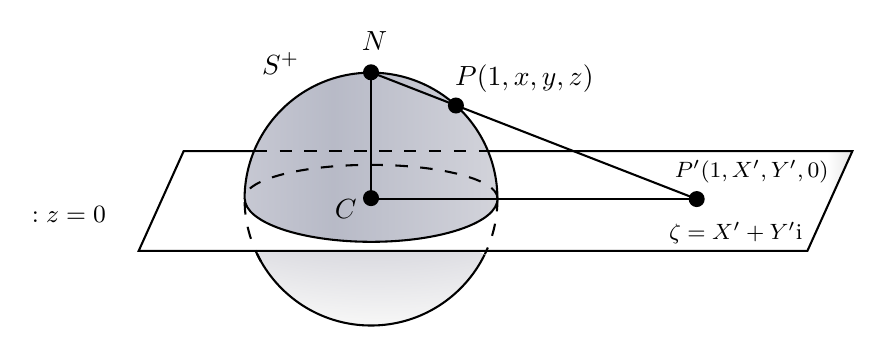
\begin{tikzpicture}[x=0.75pt,y=0.75pt,yscale=-1,xscale=1]
	%uncomment if require: \path (0,152); %set diagram left start at 0, and has height of 152
	
	%Shape: Arc [id:dp7778812556944477] 
	\draw  [draw opacity=0][shading=_gt23p819p,_2zcujs10x] (352.66,112.84) .. controls (342.75,133.07) and (321.96,147) .. (297.92,147) .. controls (273.72,147) and (252.81,132.89) .. (242.99,112.45) -- (297.92,86.08) -- cycle ; \draw   (352.66,112.84) .. controls (342.75,133.07) and (321.96,147) .. (297.92,147) .. controls (273.72,147) and (252.81,132.89) .. (242.99,112.45) ;  
	%Shape: Parallelogram [id:dp14729101837402525] 
	\path  [shading=_zhaeh0lf2,_ke7fkjhbt] (207.64,63) -- (529.83,63) -- (508.19,111) -- (186,111) -- cycle ; % for fading 
	\draw   (207.64,63) -- (529.83,63) -- (508.19,111) -- (186,111) -- cycle ; % for border 
	
	%Shape: Arc [id:dp009547815145512395] 
	\draw  [draw opacity=0][dash pattern={on 4.5pt off 4.5pt}] (358.83,86.02) .. controls (358.83,86.04) and (358.83,86.06) .. (358.83,86.08) .. controls (358.83,95.59) and (356.65,104.59) .. (352.77,112.61) -- (297.92,86.08) -- cycle ; \draw  [dash pattern={on 4.5pt off 4.5pt}] (358.83,86.02) .. controls (358.83,86.04) and (358.83,86.06) .. (358.83,86.08) .. controls (358.83,95.59) and (356.65,104.59) .. (352.77,112.61) ;  
	%Shape: Arc [id:dp2605619902920453] 
	\draw  [draw opacity=0][dash pattern={on 4.5pt off 4.5pt}] (244.93,116.16) .. controls (239.88,107.29) and (237,97.02) .. (237,86.08) .. controls (237,84.97) and (237.03,83.86) .. (237.09,82.76) -- (297.92,86.08) -- cycle ; \draw  [dash pattern={on 4.5pt off 4.5pt}] (244.93,116.16) .. controls (239.88,107.29) and (237,97.02) .. (237,86.08) .. controls (237,84.97) and (237.03,83.86) .. (237.09,82.76) ;  
	%Shape: Arc [id:dp014360101618336563] 
	\draw  [draw opacity=0][shading=_nhbclds00,_ivori3i8z] (237,86.14) .. controls (237,86.12) and (237,86.1) .. (237,86.08) .. controls (237,52.44) and (264.27,25.17) .. (297.92,25.17) .. controls (331.43,25.17) and (358.63,52.23) .. (358.83,85.7) -- (297.92,86.08) -- cycle ; \draw   (237,86.14) .. controls (237,86.12) and (237,86.1) .. (237,86.08) .. controls (237,52.44) and (264.27,25.17) .. (297.92,25.17) .. controls (331.43,25.17) and (358.63,52.23) .. (358.83,85.7) ;  
	%Shape: Arc [id:dp5813015502811212] 
	\draw  [draw opacity=0][shading=_icebnqz8w,_jlfrhqr83] (358.92,85.75) .. controls (358.92,85.77) and (358.92,85.8) .. (358.92,85.83) .. controls (358.92,97.34) and (331.65,106.67) .. (298,106.67) .. controls (264.36,106.67) and (237.09,97.34) .. (237.09,85.83) .. controls (237.09,85.81) and (237.09,85.78) .. (237.09,85.76) -- (298,85.83) -- cycle ; \draw   (358.92,85.75) .. controls (358.92,85.77) and (358.92,85.8) .. (358.92,85.83) .. controls (358.92,97.34) and (331.65,106.67) .. (298,106.67) .. controls (264.36,106.67) and (237.09,97.34) .. (237.09,85.83) .. controls (237.09,85.81) and (237.09,85.78) .. (237.09,85.76) ;  
	%Straight Lines [id:da5221405117017395] 
	\draw  [dash pattern={on 4.5pt off 4.5pt}]  (241.83,63) -- (353.83,63) ;
	%Straight Lines [id:da24524464444311378] 
	\draw    (297.92,25) -- (454.83,86.08) ;
	%Shape: Arc [id:dp550601865905674] 
	\draw  [draw opacity=0][dash pattern={on 4.5pt off 4.5pt}] (358.83,85.7) .. controls (358.83,85.67) and (358.83,85.64) .. (358.83,85.62) .. controls (358.83,76.76) and (331.56,69.59) .. (297.92,69.59) .. controls (264.27,69.59) and (237,76.76) .. (237,85.62) .. controls (237,85.64) and (237,85.67) .. (237,85.69) -- (297.92,85.62) -- cycle ; \draw  [dash pattern={on 4.5pt off 4.5pt}] (358.83,85.7) .. controls (358.83,85.67) and (358.83,85.64) .. (358.83,85.62) .. controls (358.83,76.76) and (331.56,69.59) .. (297.92,69.59) .. controls (264.27,69.59) and (237,76.76) .. (237,85.62) .. controls (237,85.64) and (237,85.67) .. (237,85.69) ;  
	%Straight Lines [id:da047382324055451175] 
	\draw    (297.92,86.08) -- (454.83,86.08) ;
	\draw [shift={(454.83,86.08)}, rotate = 0] [color={rgb, 255:red, 0; green, 0; blue, 0 }  ][fill={rgb, 255:red, 0; green, 0; blue, 0 }  ][line width=0.75]      (0, 0) circle [x radius= 3.35, y radius= 3.35]   ;
	%Straight Lines [id:da4398538993246077] 
	\draw    (297.92,25) -- (297.92,85.62) ;
	\draw [shift={(297.92,85.62)}, rotate = 90] [color={rgb, 255:red, 0; green, 0; blue, 0 }  ][fill={rgb, 255:red, 0; green, 0; blue, 0 }  ][line width=0.75]      (0, 0) circle [x radius= 3.35, y radius= 3.35]   ;
	\draw [shift={(297.92,25)}, rotate = 90] [color={rgb, 255:red, 0; green, 0; blue, 0 }  ][fill={rgb, 255:red, 0; green, 0; blue, 0 }  ][line width=0.75]      (0, 0) circle [x radius= 3.35, y radius= 3.35]   ;
	%Straight Lines [id:da9917829639130094] 
	\draw    (338.83,41) ;
	\draw [shift={(338.83,41)}, rotate = 0] [color={rgb, 255:red, 0; green, 0; blue, 0 }  ][fill={rgb, 255:red, 0; green, 0; blue, 0 }  ][line width=0.75]      (0, 0) circle [x radius= 3.35, y radius= 3.35]   ;
	
	
	% Text Node
	\draw (440,95.96) node [anchor=north west][inner sep=0.75pt]  [font=\footnotesize]  {$\zeta =X'+Y'\mathrm{i}$};
	% Text Node
	\draw (133,88) node [anchor=north west][inner sep=0.75pt]  [font=\small]  {$\upSigma :z=0$};
	% Text Node
	\draw (244,14) node [anchor=north west][inner sep=0.75pt]    {$S^{+}$};
	% Text Node
	\draw (292,4) node [anchor=north west][inner sep=0.75pt]    {$N$};
	% Text Node
	\draw (337,20) node [anchor=north west][inner sep=0.75pt]    {$P( 1,x,y,z)$};
	% Text Node
	\draw (279,85) node [anchor=north west][inner sep=0.75pt]    {$C$};
	% Text Node
	\draw (442.83,66.08) node [anchor=north west][inner sep=0.75pt]  [font=\footnotesize]  {$P'( 1,X',Y',0)$};
	
	
\end{tikzpicture}
	\caption{球极投影将天球上的点映射到复平面$\mathbb{C} \cup \{\infty \}$上,其中北极点映射到复平面的无穷远点。}
	\label{fig:argand-plane}
\end{figure}

如图\ref{fig:argand-plane}所示,我们可以用一个复数$\zeta $将平面$\upSigma :z=0$参数化:
\begin{equation*}
	\zeta =X'+\mathrm{i} Y'.
\end{equation*}
很容易用初中几何计算出
\begin{equation*}
	\zeta =\frac{x+\mathrm{i} y}{1-z} .
\end{equation*}
我们也很容易给出逆,观察到
\begin{equation*}
	\zeta \overline{\zeta } =\frac{1+z}{1-z} ,
\end{equation*}
这意味着
\begin{equation}
	x=\frac{\zeta +\overline{\zeta }}{\zeta \overline{\zeta } +1} ,\quad y=\frac{\zeta -\overline{\zeta }}{\mathrm{i} (\zeta \overline{\zeta } +1)} ,\quad z=\frac{\zeta \overline{\zeta } -1}{\zeta \overline{\zeta } +1} .
	\label{eq:coordinate of stereographic projection}
\end{equation}
如果我们用球坐标参数化$x,y,z$:
\begin{equation*}
	x=\sin \theta \cos \phi ,\quad y=\sin \theta \sin \phi ,\quad z=\cos \theta ,
\end{equation*}
我们可以给出:
\begin{equation*}
	\zeta =\mathrm{e}^{\mathrm{i} \phi }\cot\frac{\theta }{2} .
\end{equation*}
对于$S^{-}$,我们只需要做一个对顶点映射(antipodal map)$( x,y,z) \mapsto -(x,y,z )$或者$( \theta ,\phi ) \mapsto ( \pi -\theta ,\pi +\phi )$,这样我们就有
\begin{equation*}
	\zeta =-\mathrm{e}^{\mathrm{i} \phi }\tan\frac{\theta }{2} .
\end{equation*}

\subsection{洛伦兹变换与自旋变换*}

除了用非齐次坐标$\zeta $来刻画$S^{+}$上的点,我们也可以用齐次坐标$( \xi ,\eta )$来刻画一个复数:
\begin{equation*}
	\zeta =\frac{\xi }{\eta } .
\end{equation*}
这里$( \lambda \xi ,\lambda \eta )$为同一个点。在齐次坐标下,我们有:
\begin{equation}
	x=\frac{\xi \overline{\eta } +\eta \overline{\xi }}{\xi \overline{\xi } +\eta \overline{\eta }} ,\quad y=\frac{\xi \overline{\eta } -\eta \overline{\xi }}{\mathrm{i} (\xi \overline{\xi } +\eta \overline{\eta } )} ,\quad z=\frac{\xi \overline{\xi } -\eta \overline{\eta }}{\xi \overline{\xi } +\eta \overline{\eta }} .
	\label{eq:homogeneous coordinate of stereoprojection}
\end{equation}
特别地,注意到我们可以选择$OP$上任意一点$R$来刻画与$OP$相同的类光方向,我们选择
\begin{equation*}
	\overrightarrow{OR} =\frac{\xi \overline{\xi } +\eta \overline{\eta }}{\sqrt{2}}\overrightarrow{OP} ,
\end{equation*}
那么我们实际上就有$\boldsymbol{K} \equiv \overrightarrow{OR}$的坐标为
\begin{equation}
	\begin{aligned}
		& T=\frac{1}{\sqrt{2}} (\xi \overline{\xi } +\eta \overline{\eta } ),\ \  & X=\frac{1}{\sqrt{2}} (\xi \overline{\eta } +\eta \overline{\xi } ),\\
		& Y=\frac{1}{\mathrm{i}\sqrt{2}} (\xi \overline{\eta } -\eta \overline{\xi } ),\ \  & Z=\frac{1}{\sqrt{2}} (\xi \overline{\xi } -\eta \overline{\eta } ).
	\end{aligned}
	\label{eq:real and complex coordinate}
\end{equation}
与点$P$不同,$R$不再有在标度变换$( \xi ,\eta ) \mapsto ( r\xi ,r\eta )$下的不变性,但仍在相位变换$( \xi ,\eta ) \mapsto (\mathrm{e}^{\mathrm{i} \theta } \xi ,\mathrm{e}^{\mathrm{i} \theta } \eta )$下不变。



现在,根据 \ref{eq:real and complex coordinate} 的形式我们可以看出,任何一个对于$( \xi ,\eta )$的复线性变换会诱导出一个$( T,X,Y,Z)$上的实线性变换。同时又注意到四个类光矢量能张成整个向量空间$\mathbb{V}$,这意味着对于类光矢量的线性变换会自然给出整个$\mathbb{V}$空间上的线性变换。不过注意,在这样的变换下,式\ref{eq:lightlike vector}是不变的,这意味着这样的变换诱导出了一个可能带有伸缩的洛伦兹变换。即,我们考虑对于$\xi ,\eta $的复线性变换:
\begin{equation*}
	\begin{aligned}
		\xi  & \mapsto \tilde{\xi } =\alpha \xi +\beta \eta \\
		\eta  & \mapsto \tilde{\eta } =\gamma \xi +\delta \eta ,
	\end{aligned}
\end{equation*}
其中$\alpha ,\beta ,\gamma ,\delta \in \mathbb{C}$。为了保证这个线性变换非奇异,我们只需要要求$\alpha \delta -\beta \gamma \neq 0$即可。用复数$\zeta $表达,这个变换等价于
\begin{equation*}
	\zeta \mapsto \tilde{\zeta } =\frac{\alpha \zeta +\beta }{\gamma \zeta +\delta } .
\end{equation*}
如果我们加上一个归一化条件:
\begin{equation*}
	\alpha \delta -\beta \gamma =1,
\end{equation*}
那么我们称这样的变换为\textbf{自旋变换}(spin transformation)。同样的,我们也可以定义一个\textbf{自旋矩阵}$\boldsymbol{A}$为:
\begin{equation*}
	\boldsymbol{A} \equiv \begin{pmatrix}
		\alpha  & \beta \\
		\gamma  & \delta 
	\end{pmatrix} ,\det\boldsymbol{A} =1,
\end{equation*}
此时线性变换可以写成
\begin{equation*}
	\begin{pmatrix}
		\tilde{\xi }\\
		\tilde{\eta }
	\end{pmatrix} =\boldsymbol{A}\begin{pmatrix}
		\xi \\
		\eta 
	\end{pmatrix} .
\end{equation*}
显然,这样的自旋变换构成了$SL( 2,\mathbb{C})$群。但是注意,并不是一个$\zeta $的变换对应了一个自旋矩阵,因为显然$\boldsymbol{A} ,-\boldsymbol{A}$对应了同样的$\zeta $变换。如果反过来,假设存在$\boldsymbol{A} ,\boldsymbol{B}$对应了同一个$\zeta $的变换,那么$\boldsymbol{B}^{-1}\boldsymbol{A}$对应了$\zeta $的单位变换,也即$\pm \boldsymbol{I}$,因此我们知道$\boldsymbol{A} =\pm \boldsymbol{B}$。这意味着两个自旋变换对应了一个洛伦兹变换,这意味着我们可以记洛伦兹变换构成的群为$PSL( 2,\mathbb{C}) \equiv SL( 2,\mathbb{C}) /\mathbb{Z}_{2}$。



现在我们来考察自旋变换在坐标$( T,X,Y,Z)$上的效果。我们已经有了用$( \xi ,\eta )$表示$( T,X,Y,Z)$的表达式\ref{eq:real and complex coordinate},反过来我们注意到:
\begin{equation*}
	\frac{1}{\sqrt{2}}\begin{pmatrix}
		T+Z & X+\mathrm{i} Y\\
		X-\mathrm{i} Y & T-Z
	\end{pmatrix} =\begin{pmatrix}
		\xi \overline{\xi } & \xi \overline{\eta }\\
		\eta \overline{\xi } & \eta \overline{\eta }
	\end{pmatrix} =\begin{pmatrix}
		\xi \\
		\eta 
	\end{pmatrix}\begin{pmatrix}
		\overline{\xi } & \overline{\eta }
	\end{pmatrix} .
\end{equation*}
现在我们很容易看出,自旋变换的效果为
\begin{equation}
	\begin{pmatrix}
		T+Z & X+\mathrm{i} Y\\
		X-\mathrm{i} Y & T-Z
	\end{pmatrix} \mapsto \begin{pmatrix}
		\tilde{T} +\tilde{Z} & \tilde{X} +\mathrm{i}\tilde{Y}\\
		\tilde{X} -\mathrm{i}\tilde{Y} & \tilde{T} -\tilde{Z}
	\end{pmatrix} =\boldsymbol{A}\begin{pmatrix}
		T+Z & X+\mathrm{i} Y\\
		X-\mathrm{i} Y & T-Z
	\end{pmatrix}\boldsymbol{A}^{\dagger } .
	\label{eq:effect of a spin transformation}
\end{equation}
即使向量$\boldsymbol{U} =T\boldsymbol{t} +X\boldsymbol{x} +Y\boldsymbol{y} +Z\boldsymbol{z}$不是类光的,$\boldsymbol{A}$仍然诱导出了一个保证范数$T^{2} -X^{2} -Y^{2} -Z^{2}$不变的变换,因为
\begin{equation*}
	\det\begin{pmatrix}
		T+Z & X+\mathrm{i} Y\\
		X-\mathrm{i} Y & T-Z
	\end{pmatrix} =T^{2} -X^{2} -Y^{2} -Z^{2} ,
\end{equation*}
从而\ref{eq:effect of a spin transformation}定义了一个洛伦兹变换。将其转换成对于坐标$( T,X,Y,Z)$的具体形式,我们有:
\begin{equation*}
	\begin{pmatrix}
		T\\
		X\\
		Y\\
		Z
	\end{pmatrix} \mapsto \begin{pmatrix}
		\tilde{T}\\
		\tilde{X}\\
		\tilde{Y}\\
		\tilde{Z}
	\end{pmatrix} =\frac{1}{2}\boldsymbol{B}\begin{pmatrix}
		T\\
		X\\
		Y\\
		Z
	\end{pmatrix} ,
\end{equation*}
其中
\begin{equation*}
	\begin{aligned}
		& \boldsymbol{B} =\\
		& {\small\begin{pmatrix}
				\alpha \overline{\alpha } +\beta \overline{\beta } +\gamma \overline{\gamma } +\delta \delta  & \alpha \overline{\beta } +\beta \overline{\alpha } +\gamma \delta +\delta \overline{\gamma } & \mathrm{i} (\alpha \beta -\beta \overline{\alpha } +\gamma \overline{\delta } -\delta \overline{\gamma } ) & \alpha \overline{\alpha } -\beta \overline{\beta } +\gamma \overline{\gamma } -\delta \overline{\delta }\\
				\alpha \overline{\gamma } +\gamma \overline{\alpha } +\beta \overline{\delta } +\delta \overline{\beta } & \alpha \delta +\delta \overline{\alpha } +\beta \overline{\gamma } +\gamma \beta  & \mathrm{i} (\alpha \delta -\delta \overline{\alpha } +\gamma \overline{\beta } -\beta \overline{\gamma } ) & \alpha \overline{\gamma } +\gamma \overline{\alpha } -\beta \delta -\delta \beta \\
				\mathrm{i} (\gamma \overline{\alpha } -\alpha \overline{\gamma } +\delta \overline{\beta } -\beta \overline{\delta } ) & \mathrm{i} (\delta \overline{\alpha } -\alpha \delta +\gamma \beta -\beta \overline{\gamma } ) & \alpha \delta +\delta \overline{\alpha } -\beta \overline{\gamma } -\gamma \overline{\beta } & \mathrm{i} (\gamma \overline{\alpha } -\alpha \overline{\gamma } +\beta \overline{\delta } -\delta \overline{\beta } )\\
				\alpha \overline{\alpha } +\beta \overline{\beta } -\gamma \overline{\gamma } -\delta \delta  & \alpha \beta +\beta \overline{\alpha } -\gamma \delta -\delta \overline{\gamma } & \mathrm{i} (\alpha \beta -\beta \overline{\alpha } +\delta \overline{\gamma } -\gamma \delta ) & \alpha \overline{\alpha } -\beta \overline{\beta } -\gamma \overline{\gamma } +\delta \overline{\delta }
		\end{pmatrix}} .
	\end{aligned}
\end{equation*}
注意,这一定是一个限制性洛伦兹变换,因为$\boldsymbol{A}$与单位元连通,而且即使$\boldsymbol{A} =-\boldsymbol{I}$,我们也可以通过自旋变换$\operatorname{diag} (\mathrm{e}^{\mathrm{i} \theta } ,\mathrm{e}^{-\mathrm{i} \theta } )$将其变为$\boldsymbol{I}$。

总结上面的内容,这意味着我们有以下结论:


\begin{them}[label={them:Spin and Lorentz transformation}]{自旋变换与洛伦兹变换的对应关系}
	每一个自旋变换对应了一个限制性洛伦兹变换;反过来一个限制性洛伦兹变换对应了两个自旋变换,这两个自旋变换相差一个负号。
\end{them}

除此之外,我们知道一个洛伦兹变换可以由旋转与推动生成,那么旋转和推动对应了什么样的自旋变换呢?我们给出下面这样的定理:

\begin{them}[label={them:rotation and spin transformation}]{旋转与自旋变换}
	每一个\textbf{幺正}的自旋变换对应了一个$S^{+}$上的正当旋转,而反过来每一个$S^{+}$上的正当旋转也对应了两个互为相反的幺正自旋变换。
\end{them}

现在我们来证明定理\ref{them:rotation and spin transformation}。首先需要澄清的是,$S^{+}$上的旋转在定义上并不等价于洛伦兹变换中的旋转,但由于洛伦兹变换中的旋转改变了闵氏向量空间中的矢量的方向,而每一个指向未来的类光方向被旋转代表着它在$S^{+}$上对应的点也旋转了,因此我们可以不严谨地称其为$S^{+}$上的旋转。这里的关键仍然在于,我们只是旋转了$\mathbb{V}$中的类光矢量,但是正是由于类光矢量构成了$\mathbb{V}$中的一个基,因此它们的变换对应了$\mathbb{V}$中所有向量的变换。

现在根据\ref{eq:effect of a spin transformation},我们发现在幺正自旋变换下$T$是不变的,因为
\begin{equation*}
	\begin{aligned}
		& \operatorname{tr}\begin{pmatrix}
			T+Z & X+\mathrm{i} Y\\
			X-\mathrm{i} Y & T-Z
		\end{pmatrix} =2T\\
		\mapsto  & \operatorname{tr}\boldsymbol{A}\begin{pmatrix}
			T+Z & X+\mathrm{i} Y\\
			X-\mathrm{i} Y & T-Z
		\end{pmatrix}\boldsymbol{A}^{\dagger } =\operatorname{tr}\begin{pmatrix}
			T+Z & X+\mathrm{i} Y\\
			X-\mathrm{i} Y & T-Z
		\end{pmatrix} .
	\end{aligned}
\end{equation*}
我们又知道,保证$T$不变的限制性洛伦兹变换就是正规旋转,因此我们证明了定理\ref{them:rotation and spin transformation}的前半部分。要证明定理\ref{them:rotation and spin transformation}的后半部分,我们可以将任意一个旋转用欧拉角分解成绕$y$轴和绕$z$轴的旋转,只要我们分别给出两种旋转对应的自旋变换,我们就证明了这个定理。考虑绕$z$的旋转,我们从Argand平面可以看出,绕$z$轴的旋转等价于
\begin{equation*}
	\tilde{\zeta } =\mathrm{e}^{\mathrm{i} \psi } \zeta ,
\end{equation*}
即对应自旋变换
\begin{equation*}
	\begin{pmatrix}
		\tilde{\xi }\\
		\tilde{\eta }
	\end{pmatrix} =\pm \begin{pmatrix}
		\mathrm{e}^{\mathrm{i} \psi /2} & 0\\
		0 & \mathrm{e}^{-\mathrm{i} \psi /2}
	\end{pmatrix}\begin{pmatrix}
		\xi \\
		\eta 
	\end{pmatrix} .
\end{equation*}
现在我们考虑绕$y$轴的旋转,我们考虑幺正变换:
\begin{equation*}
	\begin{pmatrix}
		\tilde{\xi }\\
		\tilde{\eta }
	\end{pmatrix} =\pm \begin{pmatrix}
		\cos\frac{\theta }{2} & -\sin\frac{\theta }{2}\\
		\sin\frac{\theta }{2} & \cos\frac{\theta }{2}
	\end{pmatrix}\begin{pmatrix}
		\xi \\
		\eta 
	\end{pmatrix} ,
\end{equation*}
由于它是幺正变换,那么它一定对应某个旋转。但同时我们又可以看出这个变换保证$\xi \overline{\eta } -\eta \overline{\xi }$和$\xi \overline{\xi } +\eta \overline{\eta }$不变,从\ref{eq:coordinate of stereographic projection}我们可以看出$y$轴的坐标也不变,因此这是绕$y$轴的旋转。同时,我们可以发现这个变换将点$( 1,0,0,1)$变换到$( 1,\sin \theta ,0,\cos \theta )$,因此这个旋转的转角为$\theta $。因此,对于一般的欧拉角为$\theta ,\phi ,\psi $的旋转,其对应的自旋矩阵为
\begin{equation*}
	\pm \begin{pmatrix}
		\cos\frac{\theta }{2}\mathrm{e}^{\mathrm{i} (\phi +\psi )/2} & -\sin\frac{\theta }{2}\mathrm{e}^{\mathrm{i} (\phi -\psi )/2}\\
		\sin\frac{\theta }{2}\mathrm{e}^{-\mathrm{i} (\phi -\psi )/2} & \cos\frac{\theta }{2}\mathrm{e}^{-\mathrm{i} (\phi +\psi )/2}
	\end{pmatrix} .
\end{equation*}
这意味着我们成功证明了定理\ref{them:rotation and spin transformation}。



刚才考虑了旋转,那么推动对应了什么样的自旋变换呢?由于任何推动都可以被分解成到$z$轴的旋转-$z$方向的推动-旋转回去,因此我们只需考虑$z$方向的推动:
\begin{equation*}
	\begin{cases}
		\tilde{T} +\tilde{Z} & =w(T+Z)\\
		\tilde{T} -\tilde{Z} & =w^{-1} (T-Z)\\
		\tilde{X} & =X\\
		\tilde{Y} & =Y
	\end{cases}
\end{equation*}


其中
\begin{equation*}
	w=\left(\frac{1+v}{1-v}\right)^{1/2} .
\end{equation*}
这对应了自旋变换
\begin{equation*}
	\begin{pmatrix}
		\tilde{\xi }\\
		\tilde{\eta }
	\end{pmatrix} =\pm \begin{pmatrix}
		w^{1/2} & 0\\
		0 & w^{-1/2}
	\end{pmatrix}\begin{pmatrix}
		\xi \\
		\eta 
	\end{pmatrix} .
\end{equation*}
在Argand平面上,我们有
\begin{equation*}
	\tilde{\zeta } =w\zeta .
\end{equation*}
对于一般的推动,其对应的自旋变换为正定的厄米矩阵。

\section{洛伦兹变换的性质*}

现在,我们可以利用自旋变换非常简便地导出洛伦兹变换的许多性质。

\begin{prop}[label={prop:fixed point of rotation}]{旋转的不动点}
	球面$S^{+} /S^{-}$上的任意旋转有两个不动点,为球面的对顶点,这意味着每一个旋转都等价于绕着一个轴的旋转。
\end{prop}


\begin{proof}
	由于每一个旋转都是幺正的,我们可以将自旋变换写成
	\begin{equation*}
		\tilde{\zeta } =\frac{\alpha \zeta -\overline{\gamma }}{\gamma \zeta +\overline{\alpha }} ,
	\end{equation*}
	那么其不动点$\tilde{\zeta } =\zeta $就为
	\begin{equation*}
		\gamma \zeta ^{2} +(\overline{\alpha } -\alpha )\zeta +\overline{\gamma } =0.
	\end{equation*}
	注意到如果$\zeta $为这个方程的一个根,那么$-1/\overline{\zeta }$则为另一个根,而根据
	\begin{equation*}
		\zeta =-\mathrm{e}^{\mathrm{i} \phi }\tan \theta /2\Rightarrow -\frac{1}{\overline{\zeta }} =-\mathrm{e}^{\mathrm{i} (\pi +\phi )}\tan\frac{\pi -\theta }{2} ,
	\end{equation*}
	这意味着两个不动点为$S^{+}$上的对顶点。
\end{proof}

除此之外,一般的自旋变换也仅仅只有两个不动点,这意味着每一个(非平凡)洛伦兹变换也只能保证两个类光方向不变。事实上,根据庞加莱-霍普夫定理,每一个保持定向到黎曼球面自身的连续映射一定会至少有一个不动点,而由于$S^{2}$的欧拉数是$2$,这意味着这样的映射的映射度也是$2$。



下面我们考虑一般的洛伦兹变换,如果我们令$\boldsymbol{t} ,\boldsymbol{z}$两个不变的类光方向张成的平面上,那么实际上我们知道这个变换的不动点在$S^{+}$的两极。这种变换的最一般形式可以被写成
\begin{equation*}
	\tilde{\zeta } =w\mathrm{e}^{\mathrm{i} \psi } \zeta ,
\end{equation*}
即绕$z$轴的旋转与推动的复合,并且我们称这种变换为four-screw。图\ref{fig:visualization of lorentz transformation}是将旋转,推动以及four-screw变换可视化后的结果。

\begin{figure}[h]
	\centering
	

\tikzset{every picture/.style={line width=0.75pt}} %set default line width to 0.75pt        

\begin{tikzpicture}[x=0.75pt,y=0.75pt,yscale=-1,xscale=1]
	%uncomment if require: \path (0,475); %set diagram left start at 0, and has height of 475
	
	%Image [id:dp211355850900945] 
	\draw (169.86,117.75) node  {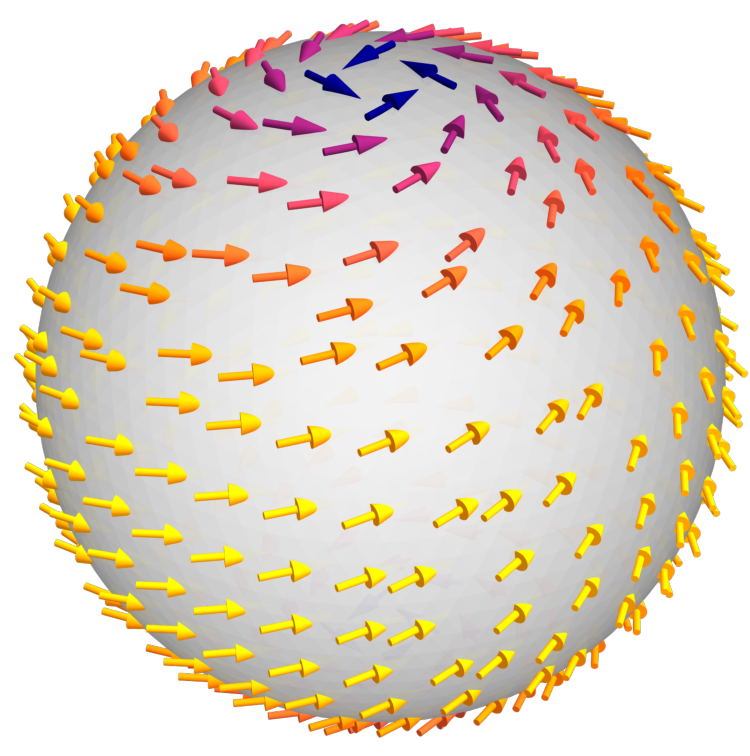
\includegraphics[width=160.28pt,height=161.62pt]{rotation.pdf}};
	
	%Image [id:dp48213474837212833] 
	\draw (474.86,115.75) node  {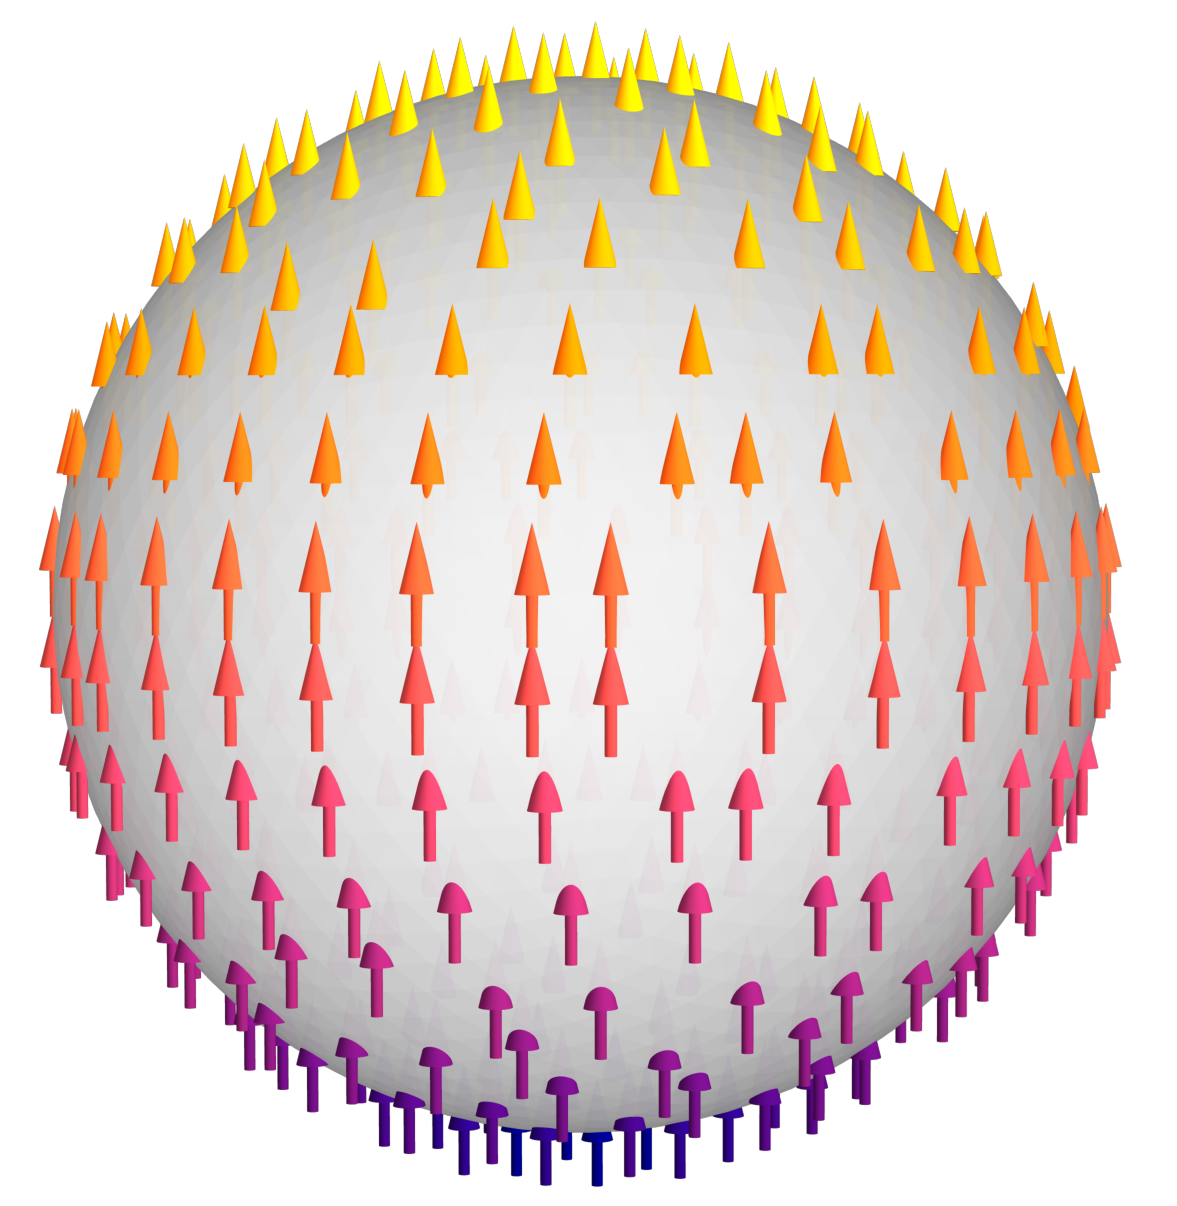
\includegraphics[width=160.28pt,height=161.62pt]{boost.pdf}};
	
	%Image [id:dp180039259569454] 
	\draw (324.5,335.25) node  {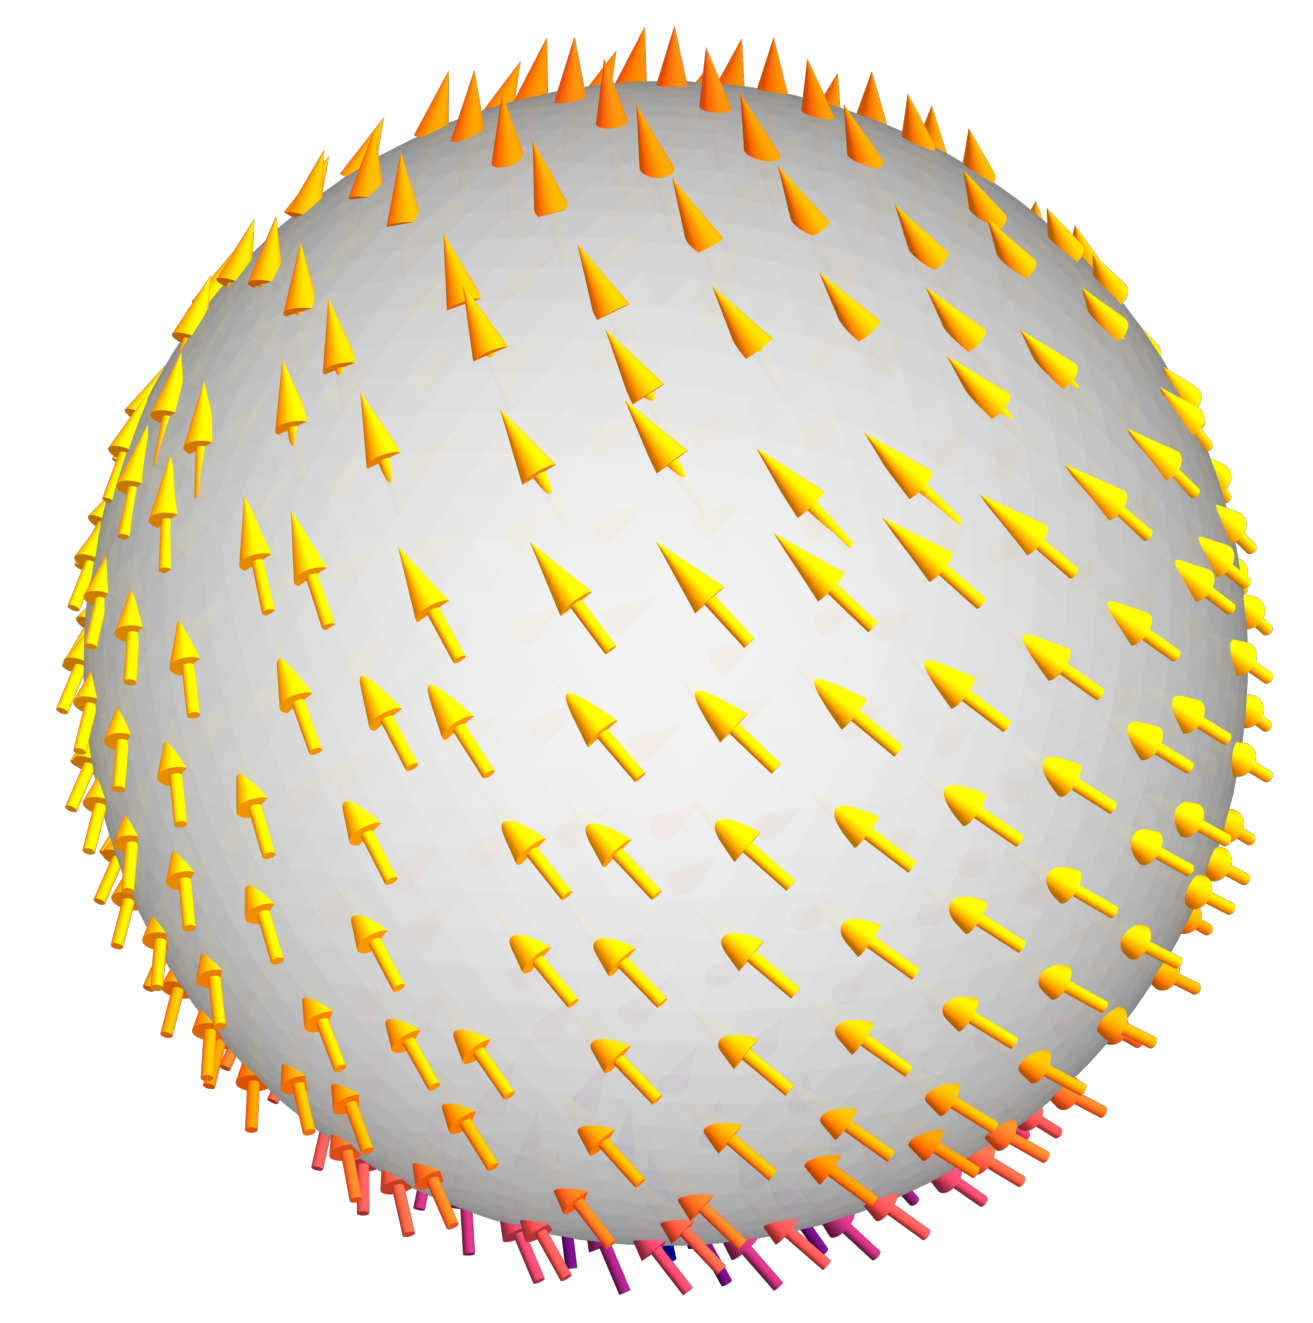
\includegraphics[width=170.25pt,height=159.37pt]{four screw.pdf}};
	
	%Straight Lines [id:da15923397993352584] 
	\draw    (289,117.22) -- (360.7,117.22) ;
	%Straight Lines [id:da09146095317161684] 
	\draw    (324.85,117.22) -- (324.85,227.23) ;
	\draw [shift={(324.85,230.23)}, rotate = 270] [fill={rgb, 255:red, 0; green, 0; blue, 0 }  ][line width=0.08]  [draw opacity=0] (10.72,-5.15) -- (0,0) -- (10.72,5.15) -- (7.12,0) -- cycle    ;
	
	% Text Node
	\draw (249,452) node [anchor=north west][inner sep=0.75pt]   [align=left] {effect of a four-screw};
	% Text Node
	\draw (103,233) node [anchor=north west][inner sep=0.75pt]   [align=left] {effect of a rotation};
	% Text Node
	\draw (414,234) node [anchor=north west][inner sep=0.75pt]   [align=left] {effect of a boost};
	
	
\end{tikzpicture}
	\caption{将不同洛伦兹变换在黎曼球上可视化}
	\label{fig:visualization of lorentz transformation}
\end{figure}

如果洛伦兹变换保持不变的两个类光方向重合,那么我们将这种情况称作类光旋转(null rotation)。我们可以将不动点定为$\zeta =\infty $,这时自旋变换就为
\begin{equation*}
	\tilde{\zeta } =\zeta +\beta ,
\end{equation*}
自旋变换矩阵就为
\begin{equation*}
	\begin{pmatrix}
		\tilde{\xi }\\
		\tilde{\eta }
	\end{pmatrix} =\pm \begin{pmatrix}
		1 & \beta \\
		0 & 1
	\end{pmatrix}\begin{pmatrix}
		\xi \\
		\eta 
	\end{pmatrix} .
\end{equation*}
其可视化效果如图\ref{fig:visualization of null rotation}所示。

\begin{figure}[h]
	\centering
	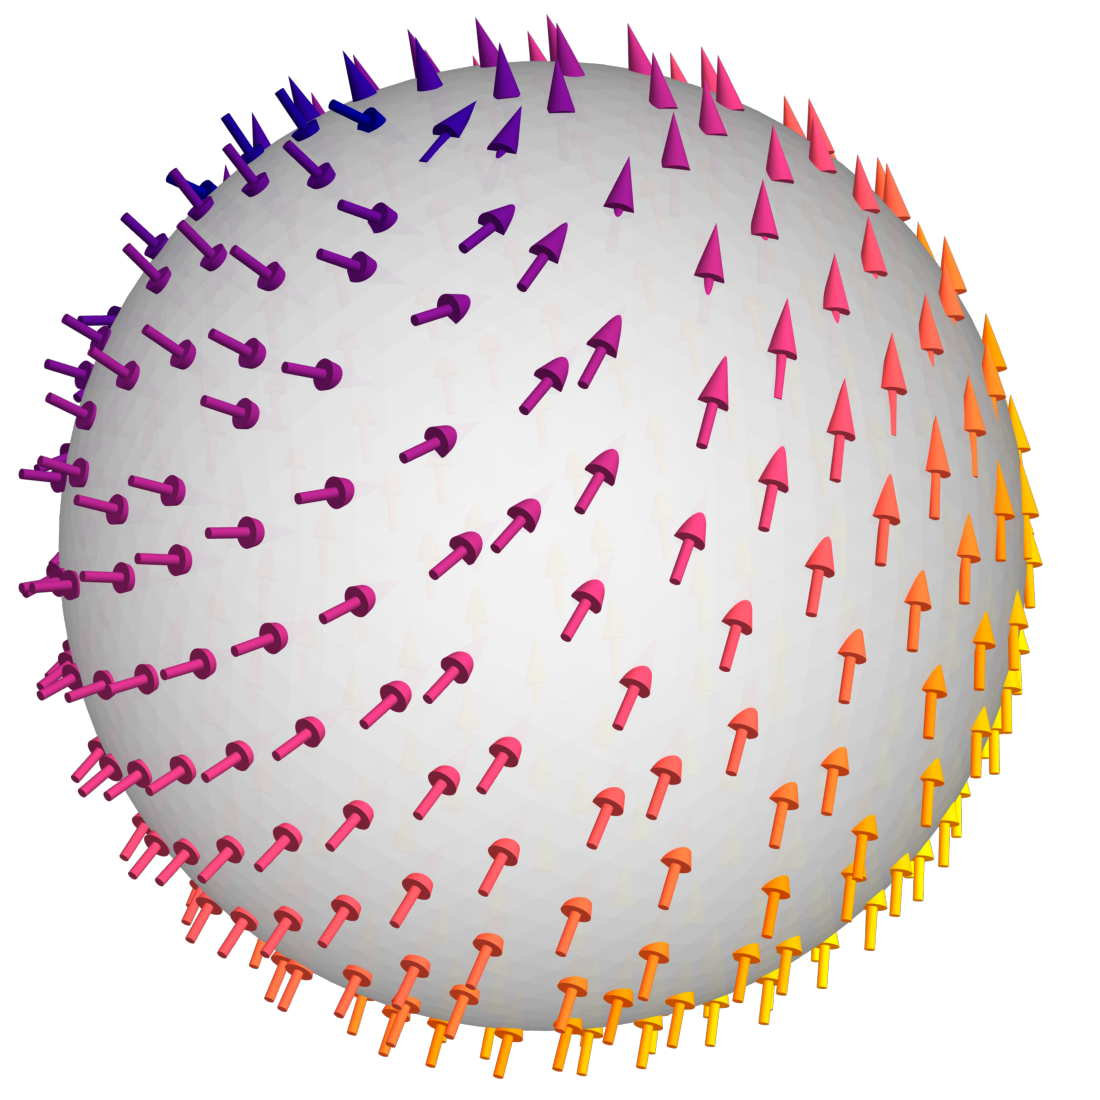
\includegraphics[width=160.28pt,height=161.62pt]{null rotation.pdf}
	\caption{类光旋转可视化化}
	\label{fig:visualization of null rotation}
\end{figure}

\section{类光旗帜与自旋矢量*}

本节的目的是让我们对自旋矢量有一个直观的几何理解。我们知道复数对$( \xi ,\eta )$定义了一个自旋矢量$\boldsymbol{\kappa }$,这与闵氏向量空间中的类光矢量$\boldsymbol{K}$有对应关系\ref{eq:real and complex coordinate}。但我们知道如果用$( \xi ,\eta )$作为$\boldsymbol{K}$的坐标,有冗余自由度$\xi \mapsto \mathrm{e}^{\mathrm{i} \theta } \xi ,\eta \mapsto \mathrm{e}^{\mathrm{i} \theta } \eta $。这个变换很容易让我们想到三维空间中的旋转,因此我们想要将这个冗余自由度阐释为一个“几何结构”,在这个结构之外,多余的自由度可以被缩减到一个符号的不确定性。这个几何结构就是所谓\textbf{类光旗帜}(null flag),即$\boldsymbol{K}$能对应到一个平面相位意义上的$\xi ,\eta $,我们只需要考虑这个“旗帜面”。



除此之外,注意我们所寻找的$( \xi ,\eta )$的几何结构是“内禀”的,即不依赖于坐标的选取。例如考虑自旋变换诱导的被动洛伦兹变换,这样的变换并不会改变$\boldsymbol{\kappa }$的几何结构。



我们的思路是首先在所有类光方向的曲面$\mathcal{S}^{+}$上描述$( \xi ,\eta )$的几何结构,随后再将其引入到$\mathbb{V}$上。


\subsection{$S^{+}$上的描述}

我们知道$\mathcal{S}^{+}$上的点可以与复数$\zeta \equiv \xi /\eta $一一对应,但除了这个比值之外,如果我们知道了表示$\zeta $的点$P$处的实切向量$\mathbf{L}$,那么$\xi ,\eta $也能独立地被表示出来。我们知道$\mathcal{S}^{+}$(的切空间)上的实的切向量可以被表示为
\begin{equation*}
	\mathbf{L} =\lambda \frac{\partial }{\partial \zeta } +\overline{\lambda }\frac{\partial }{\partial \overline{\zeta }} ,
\end{equation*}
其中我们需要选择系数让$\mathbf{L}$是实的。如果$\lambda ( \xi ,\eta )$可以表示为$\xi ,\eta $的定值,这意味着我们需要$\mathbf{L}$在自旋变换下是不变的,即
\begin{equation}
	\lambda '\frac{\partial }{\partial \zeta '} +\overline{\lambda } '\frac{\partial }{\partial \overline{\zeta } '} =\lambda \frac{\partial }{\partial \zeta } +\overline{\lambda }\frac{\partial }{\partial \overline{\zeta }} ,
	\label{eq:invariance of L}
\end{equation}
其中
\begin{equation*}
	\zeta '=\frac{\xi '}{\eta '} =\frac{\alpha \xi +\beta \eta }{\gamma \xi +\delta \eta } =\frac{\alpha \zeta +\beta }{\gamma \zeta +\delta } .
\end{equation*}
那么利用链式法则:
\begin{equation}
	\frac{\partial }{\partial \zeta } =\frac{\partial \zeta '}{\partial \zeta }\frac{\partial }{\partial \zeta '} =\frac{\alpha \delta -\beta \gamma }{(\delta +\gamma \zeta )^{2}}\frac{\partial }{\partial \zeta '} =(\delta +\gamma \zeta )^{-2}\frac{\partial }{\partial \zeta '} =\eta ^{2} \eta ^{\prime -2}\frac{\partial }{\partial \zeta '} .
	\label{eq:chain rule of xi}
\end{equation}
代回\ref{eq:invariance of L}并要求系数相等,我们有
\begin{equation*}
	\lambda '( \xi ',\eta ') \eta ^{\prime 2} =\lambda ( \xi ,\eta ) \eta ^{2} ,
\end{equation*}
这意味着我们必须要求$\lambda $对$\eta $的依赖关系为某个数字乘以$\eta ^{-2}$.我们选取
\begin{equation*}
	\lambda =-\frac{1}{\sqrt{2}} \eta ^{-2} ,
\end{equation*}
那么我们有
\begin{equation}
	\mathbf{L} =-\frac{1}{\sqrt{2}}\left( \eta ^{-2}\frac{\partial }{\partial \zeta } +\overline{\eta }^{-2}\frac{\partial }{\partial \overline{\zeta }}\right) .
	\label{eq:expression of L}
\end{equation}


反过来,如果我们知道$P$点以及$P$点处的$\mathbf{L}$,那么我们就可以将$( \zeta ,\eta )$确定到相差一个符号。因为通过$\mathbf{L}$的具体形式\ref{eq:expression of L},我们可以对比系数给出$\eta ^{2}$,根据$P$我们可以知道$\zeta $,从而反推出$\pm ( \xi ,\eta )$。



等价地,我们可以根据
\begin{equation*}
	\eta ^{2}\mathrm{d} \zeta =\eta \mathrm{d} \xi -\xi \mathrm{d} \eta ,
\end{equation*}
给出
\begin{equation*}
	\eta ^{\prime 2}\mathrm{d} \zeta '=\eta ^{2}\mathrm{d} \zeta ,
\end{equation*}
这与\ref{eq:chain rule of xi}等价。


\subsection{$\mathbb{V}$上的表述}

$\mathcal{S}^{+}$上的切向量$\mathbf{L}$自然诱导出了作为子空间的$S^{+}$上的切向量$\boldsymbol{L}$,而$S^{+}$上的坐标通过\ref{eq:coordinate of stereographic projection}自然与$\mathbb{V}$中的坐标相联系,那么我们可以写出
\begin{equation*}
	\boldsymbol{L} =-\frac{1}{\sqrt{2}}\left( \eta ^{-2}\frac{\partial }{\partial \zeta } +\overline{\eta }^{-2}\frac{\partial }{\partial \overline{\zeta }}\right) =L^{a}\frac{\partial }{\partial x^{a}} ,
\end{equation*}
其中$x^{a}$是$\mathbb{V}$中的坐标。选定参数$x^{0} =1$,通过\ref{eq:coordinate of stereographic projection},我们知道
\begin{equation*}
	\frac{\partial x^{0}}{\partial \zeta } =0,\frac{\partial x^{1}}{\partial \zeta } =\frac{1-\zeta ^{2}}{(\zeta \zeta +1)^{2}} ,\frac{\partial x^{2}}{\partial \zeta } =\frac{1+\zeta ^{2}}{1(\zeta \zeta +1)^{2}} ,\frac{\partial x^{3}}{\partial \zeta } =\frac{2\zeta }{(\zeta \overline{\zeta } +1)^{2}}
\end{equation*}
根据链式法则:
\begin{equation*}
	L^{a}\frac{\partial }{\partial x^{a}} =-\frac{1}{\sqrt{2}}\left( \eta ^{-2}\frac{\partial x^{a}}{\partial \zeta } +\overline{\eta }^{-2}\frac{\partial x^{a}}{\partial \zeta }\right)\frac{\partial }{\partial x^{a}}
\end{equation*}
我们有:
\begin{equation*}
	\begin{aligned}
		L^{0} & =0, & L^{1} & =\frac{\xi ^{2} +\overline{\xi }^{2} -\eta ^{2} -\overline{\eta }^{2}}{\sqrt{2} (\xi \overline{\xi } +\eta \overline{\eta } )^{2}} ,\\
		L^{2} & =\frac{\xi ^{2} -\overline{\xi }^{2} +\eta ^{2} -\overline{\eta }^{2}}{\sqrt{2}\mathrm{i} (\xi \overline{\xi } +\eta \overline{\eta } )^{2}} , & L^{3} & =\frac{-\sqrt{2} (\xi \eta +\overline{\xi }\overline{\eta } )}{(\xi \xi +\eta \overline{\eta } )^{2}} .
	\end{aligned}
\end{equation*}
我们容易发现$\boldsymbol{L}$的范数为
\begin{equation*}
	\| \boldsymbol{L} \| =L^{a} L^{b} \eta _{ab} =\frac{-2}{(\xi \overline{\xi } +\eta \overline{\eta } )^{2}} .
\end{equation*}
注意,这和\ref{eq:homogeneous coordinate of stereoprojection}式的分母一致,也就是我们用来构造$\boldsymbol{K} \equiv \overrightarrow{OR}$的比例因子。这意味着$\boldsymbol{L}$是单位矢量,当且仅当$\boldsymbol{K}$定义了一个在$S^{+}$上的点$P$。如果$( \xi ,\eta )$与$(\tilde{\xi } ,\tilde{\eta })$两点由洛伦兹变换连接,我们很容易发现$L^{a}$之间相差的并不是洛伦兹变换,因为$\boldsymbol{L}$垂直于$S^{+}$意味着与$t$轴正交,但洛伦兹变换显然不保持这个性质。但是,$\boldsymbol{K}$与$\boldsymbol{L}$构成的平面$\hat{\upPi }$却是不变的,即它与坐标无关,因此可以被看做作$\mathbb{V}$中的几何结构。

\begin{figure}[h]
	\centering
	

% Gradient Info

\tikzset {_xfijtitct/.code = {\pgfsetadditionalshadetransform{ \pgftransformshift{\pgfpoint{-69 bp } { 489 bp }  }  \pgftransformscale{3 }  }}}
\pgfdeclareradialshading{_4ys9j1xwk}{\pgfpoint{24bp}{-192bp}}{rgb(0bp)=(0.96,0.96,0.96);
	rgb(0bp)=(0.96,0.96,0.96);
	rgb(5.25bp)=(0.86,0.86,0.89);
	rgb(12.25bp)=(0.72,0.73,0.78);
	rgb(20bp)=(0.87,0.87,0.89);
	rgb(25bp)=(0.96,0.96,0.96);
	rgb(400bp)=(0.96,0.96,0.96)}

% Gradient Info

\tikzset {_34dxukbo6/.code = {\pgfsetadditionalshadetransform{ \pgftransformshift{\pgfpoint{0 bp } { 0 bp }  }  \pgftransformrotate{0 }  \pgftransformscale{2 }  }}}
\pgfdeclarehorizontalshading{_pi2xaa4p6}{150bp}{rgb(0bp)=(0.6,0.85,1);
	rgb(37.5bp)=(0.6,0.85,1);
	rgb(62.5bp)=(0,0.5,0.5);
	rgb(100bp)=(0,0.5,0.5)}

% Gradient Info

\tikzset {_gw9u3nn4y/.code = {\pgfsetadditionalshadetransform{ \pgftransformshift{\pgfpoint{0 bp } { 0 bp }  }  \pgftransformrotate{0 }  \pgftransformscale{2 }  }}}
\pgfdeclarehorizontalshading{_2xbmbn3l0}{150bp}{rgb(0bp)=(0.6,0.85,1);
	rgb(37.5bp)=(0.6,0.85,1);
	rgb(62.5bp)=(0,0.5,0.5);
	rgb(100bp)=(0,0.5,0.5)}

% Gradient Info

\tikzset {_9byeair1q/.code = {\pgfsetadditionalshadetransform{ \pgftransformshift{\pgfpoint{0 bp } { 0 bp }  }  \pgftransformrotate{0 }  \pgftransformscale{2 }  }}}
\pgfdeclarehorizontalshading{_o1fem7bmr}{150bp}{rgb(0bp)=(0.71,0.74,0.78);
	rgb(37.5bp)=(0.71,0.74,0.78);
	rgb(46.5bp)=(0.51,0.55,0.58);
	rgb(62.5bp)=(0.16,0.2,0.23);
	rgb(100bp)=(0.16,0.2,0.23)}

% Gradient Info

\tikzset {_echxgy7iy/.code = {\pgfsetadditionalshadetransform{ \pgftransformshift{\pgfpoint{13.14 bp } { 16.79 bp }  }  \pgftransformscale{1.46 }  }}}
\pgfdeclareradialshading{_31p2pzfdp}{\pgfpoint{-16bp}{-8bp}}{rgb(0bp)=(0.97,0.97,0.97);
	rgb(0bp)=(0.97,0.97,0.97);
	rgb(25bp)=(0.72,0.73,0.78);
	rgb(400bp)=(0.72,0.73,0.78)}
\tikzset{every picture/.style={line width=0.75pt}} %set default line width to 0.75pt        

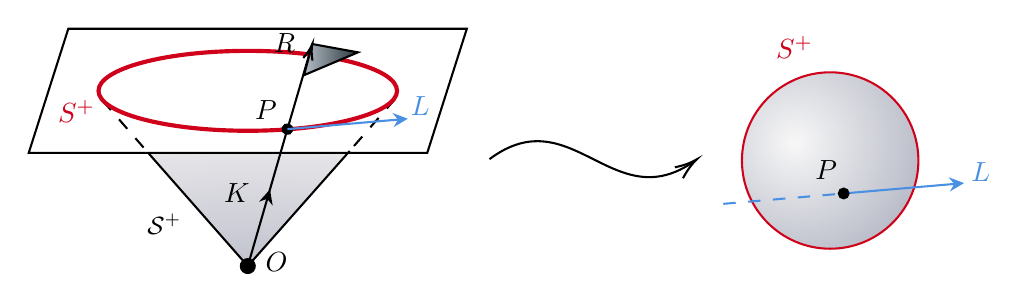
\begin{tikzpicture}[x=0.75pt,y=0.75pt,yscale=-1,xscale=1]
	%uncomment if require: \path (0,137); %set diagram left start at 0, and has height of 137
	
	%Shape: Triangle [id:dp18085529825630564] 
	\draw  [draw opacity=0][shading=_4ys9j1xwk,_xfijtitct] (203.92,121.29) -- (276.42,37.67) -- (131.41,37.67) -- cycle ;
	%Shape: Parallelogram [id:dp9228773357244249] 
	\draw  [fill={rgb, 255:red, 255; green, 255; blue, 255 }  ,fill opacity=1 ] (117.45,6.93) -- (309.46,6.93) -- (290.38,66.78) -- (98.37,66.78) -- cycle ;
	%Straight Lines [id:da7856751732458289] 
	\draw [shading=_pi2xaa4p6,_34dxukbo6]   (203.92,121.29) -- (156.01,66.83) ;
	%Straight Lines [id:da530742601835525] 
	\draw [shading=_2xbmbn3l0,_gw9u3nn4y]   (203.92,121.29) -- (253.01,65.83) ;
	\draw [shift={(203.92,121.29)}, rotate = 311.51] [color={rgb, 255:red, 0; green, 0; blue, 0 }  ][fill={rgb, 255:red, 0; green, 0; blue, 0 }  ][line width=0.75]      (0, 0) circle [x radius= 3.35, y radius= 3.35]   ;
	%Straight Lines [id:da4568538254779688] 
	\draw  [dash pattern={on 4.5pt off 4.5pt}]  (134.01,41.57) -- (156.01,66.83) ;
	%Straight Lines [id:da7131966021543883] 
	\draw  [dash pattern={on 4.5pt off 4.5pt}]  (274.83,40.85) -- (253.01,65.83) ;
	%Shape: Ellipse [id:dp8890884080819843] 
	\draw  [color={rgb, 255:red, 208; green, 2; blue, 27 }  ,draw opacity=1 ][line width=1.5]  (132,36.85) .. controls (132,26.22) and (164.2,17.6) .. (203.92,17.6) .. controls (243.64,17.6) and (275.83,26.22) .. (275.83,36.85) .. controls (275.83,47.49) and (243.64,56.1) .. (203.92,56.1) .. controls (164.2,56.1) and (132,47.49) .. (132,36.85) -- cycle ;
	%Straight Lines [id:da09373596447493804] 
	\draw    (223.01,55.31) -- (203.92,121.29) ;
	\draw [shift={(214.6,84.36)}, rotate = 106.14] [fill={rgb, 255:red, 0; green, 0; blue, 0 }  ][line width=0.08]  [draw opacity=0] (7.14,-3.43) -- (0,0) -- (7.14,3.43) -- (4.74,0) -- cycle    ;
	%Shape: Polygon [id:ds8121831694427222] 
	\path  [shading=_o1fem7bmr,_9byeair1q] (257.01,18.31) -- (231.01,29.31) -- (235.01,14.31) -- cycle ; % for fading 
	\draw   (257.01,18.31) -- (231.01,29.31) -- (235.01,14.31) -- cycle ; % for border 
	
	%Straight Lines [id:da8477468495579272] 
	\draw    (223.01,55.31) -- (234.44,16.23) ;
	\draw [shift={(235.01,14.31)}, rotate = 106.31] [color={rgb, 255:red, 0; green, 0; blue, 0 }  ][line width=0.75]    (7.65,-2.3) .. controls (4.86,-0.97) and (2.31,-0.21) .. (0,0) .. controls (2.31,0.21) and (4.86,0.98) .. (7.65,2.3)   ;
	\draw [shift={(223.01,55.31)}, rotate = 286.31] [color={rgb, 255:red, 0; green, 0; blue, 0 }  ][fill={rgb, 255:red, 0; green, 0; blue, 0 }  ][line width=0.75]      (0, 0) circle [x radius= 2.34, y radius= 2.34]   ;
	%Straight Lines [id:da15925016913815626] 
	\draw [color={rgb, 255:red, 74; green, 144; blue, 226 }  ,draw opacity=1 ]   (278.02,50.57) -- (223.01,55.31) ;
	\draw [shift={(281.01,50.31)}, rotate = 175.07] [fill={rgb, 255:red, 74; green, 144; blue, 226 }  ,fill opacity=1 ][line width=0.08]  [draw opacity=0] (7.14,-3.43) -- (0,0) -- (7.14,3.43) -- (4.74,0) -- cycle    ;
	%Curve Lines [id:da02129065464097457] 
	\draw    (320.38,69.78) .. controls (359.98,40.08) and (379.98,98.59) .. (419.19,70.65) ;
	\draw [shift={(420.38,69.78)}, rotate = 143.13] [color={rgb, 255:red, 0; green, 0; blue, 0 }  ][line width=0.75]    (10.93,-3.29) .. controls (6.95,-1.4) and (3.31,-0.3) .. (0,0) .. controls (3.31,0.3) and (6.95,1.4) .. (10.93,3.29)   ;
	%Shape: Circle [id:dp7494161810872726] 
	\path  [shading=_31p2pzfdp,_echxgy7iy] (442,70.43) .. controls (442,46.96) and (461.03,27.93) .. (484.5,27.93) .. controls (507.98,27.93) and (527.01,46.96) .. (527.01,70.43) .. controls (527.01,93.9) and (507.98,112.93) .. (484.5,112.93) .. controls (461.03,112.93) and (442,93.9) .. (442,70.43) -- cycle ; % for fading 
	\draw  [color={rgb, 255:red, 208; green, 2; blue, 27 }  ,draw opacity=1 ] (442,70.43) .. controls (442,46.96) and (461.03,27.93) .. (484.5,27.93) .. controls (507.98,27.93) and (527.01,46.96) .. (527.01,70.43) .. controls (527.01,93.9) and (507.98,112.93) .. (484.5,112.93) .. controls (461.03,112.93) and (442,93.9) .. (442,70.43) -- cycle ; % for border 
	
	%Straight Lines [id:da855599687264156] 
	\draw [color={rgb, 255:red, 74; green, 144; blue, 226 }  ,draw opacity=1 ]   (546.02,81.57) -- (491.01,86.31) ;
	\draw [shift={(549.01,81.31)}, rotate = 175.07] [fill={rgb, 255:red, 74; green, 144; blue, 226 }  ,fill opacity=1 ][line width=0.08]  [draw opacity=0] (7.14,-3.43) -- (0,0) -- (7.14,3.43) -- (4.74,0) -- cycle    ;
	%Straight Lines [id:da2554725584191] 
	\draw    (491.01,86.31) ;
	\draw [shift={(491.01,86.31)}, rotate = 0] [color={rgb, 255:red, 0; green, 0; blue, 0 }  ][fill={rgb, 255:red, 0; green, 0; blue, 0 }  ][line width=0.75]      (0, 0) circle [x radius= 2.34, y radius= 2.34]   ;
	%Straight Lines [id:da514198553655629] 
	\draw [color={rgb, 255:red, 74; green, 144; blue, 226 }  ,draw opacity=1 ] [dash pattern={on 4.5pt off 4.5pt}]  (433.01,91.31) -- (491.01,86.31) ;
	
	
	% Text Node
	\draw (211,113.5) node [anchor=north west][inner sep=0.75pt]    {$O$};
	% Text Node
	\draw (154,94.5) node [anchor=north west][inner sep=0.75pt]  [font=\small]  {$\mathcal{S}^{+}$};
	% Text Node
	\draw (111,40) node [anchor=north west][inner sep=0.75pt]  [color={rgb, 255:red, 208; green, 2; blue, 27 }  ,opacity=1 ]  {$S^{+}$};
	% Text Node
	\draw (205.92,39.85) node [anchor=north west][inner sep=0.75pt]    {$P$};
	% Text Node
	\draw (191,80) node [anchor=north west][inner sep=0.75pt]    {$\boldsymbol{K}$};
	% Text Node
	\draw (281,38) node [anchor=north west][inner sep=0.75pt]  [color={rgb, 255:red, 74; green, 144; blue, 226 }  ,opacity=1 ]  {$\boldsymbol{L}$};
	% Text Node
	\draw (215,7.94) node [anchor=north west][inner sep=0.75pt]    {$R$};
	% Text Node
	\draw (551,70) node [anchor=north west][inner sep=0.75pt]  [color={rgb, 255:red, 74; green, 144; blue, 226 }  ,opacity=1 ]  {$\boldsymbol{L}$};
	% Text Node
	\draw (475.92,68.85) node [anchor=north west][inner sep=0.75pt]    {$P$};
	% Text Node
	\draw (457,9) node [anchor=north west][inner sep=0.75pt]  [color={rgb, 255:red, 208; green, 2; blue, 27 }  ,opacity=1 ]  {$S^{+}$};
	
	
\end{tikzpicture}
	\caption{类光旗帜。注意这里$\boldsymbol{L}$并不是只有一个方向。}
	\label{fig:null flag}
\end{figure}

这里,$\hat{\upPi }$中的向量为
\begin{equation*}
	a\boldsymbol{K} +b\boldsymbol{L} ,
\end{equation*}
而我们选择$b >0$并称这个半平面为$\upPi $。我们可以看到,$\upPi $可以将$( \xi ,\eta )$决定到只差一个符号:$\boldsymbol{K}$将$\eta ,\xi $决定到相差一个全局相位,而$\boldsymbol{L}$的方向告诉我们$\eta $的相位。我们称$\upPi $与$\boldsymbol{K}$为类光旗帜(null flag)而称$\boldsymbol{K}$为旗杆(flagpole),$ $$\upPi $为旗帜面(flag plane)。



现在考虑一般的自旋变换对光旗的影响。考虑变换
\begin{equation*}
	( \xi ,\eta ) \mapsto ( \lambda \xi ,\lambda \eta ) ,\lambda \in \mathbb{C} \setminus \{0\} .
\end{equation*}
令$\lambda =r\mathrm{e}^{\mathrm{i} \theta }$,我们发现$\theta =0$时,旗帜面不变,旗杆变长$r^{2}$倍;当$r=1$时,旗杆不变,旗帜面旋转$2\theta $,因为$\boldsymbol{L}$与$\eta $呈二次相关性。



现在,如果我们考虑一个连续的旋转$( \xi ,\eta ) \mapsto (\mathrm{e}^{\mathrm{i} \theta } \xi ,\mathrm{e}^{\mathrm{i} \theta } \eta )$,其中$\theta $从$0$旋转到$\pi $,我们给出
\begin{equation*}
	( \xi ,\eta ) \mapsto ( -\xi ,-\eta ) ,
\end{equation*}
但是我们的旗帜面旋转了$2\pi $。将$\theta $继续旋转到$2\pi $,我们会给出原来的点$( \xi ,\eta )$,但旗帜面旋转了$4\pi $,这意味着如果我们想要在$\mathbb{V}$中建立一个消除符号不确定性的局域几何结构是不可能的。因为我们想要在类光旗帜中间添加的$\mathbb{V}$中的每一个局域的几何结构在旋转了$2\pi $后都会回到原来的状态,但是$( \xi ,\eta )$却会多一个全局的负号。为了更清楚地看到这一点,不妨选择$( \xi ,\eta ) =( 0,1) \mapsto (0,\mathrm{e}^{\mathrm{i} \theta } )$。当$\theta $旋转到$\pi $时,自旋变换为$-\boldsymbol{I}$,但是洛伦兹变换却是单位元,这意味着任何$V$中的几何结构都会被这个洛伦兹变换转回到它原来的状态,即使$( \xi ,\eta )$已经变成了$( -\xi ,-\eta )$。



这意味着我们应当扩充常规意义下的$\mathbb{V}$中的“几何”对象,这样的对象在旋转$2\pi $后并不回到原来的状态,当旋转$4\pi $时才回到原来的状态,这就是\textbf{旋量对象}(spinorial objects)。


\section{旋量对象与自旋结构}

众所周知,三维空间的旋转由$SO( 3)$描述,而其基本群$\pi _{1}( SO( 3)) =\mathbb{Z}_{2}$,这意味着即使\textbf{只}考虑$SO( 3)$群,我们也可以获得两种不同的“回到原点”的旋转,即旋转$2\pi $和旋转$4\pi $是$SO( 3)$的基本群中的两个元素。在$SO( 3)$的拓扑空间$\mathbb{R} P^{3}$中,旋转$2\pi $的曲线(圈)不可以被连续地变换到一个点,而旋转$4\pi $的曲线则可以。例如考虑狄拉克的皮带实验,这说明考虑旋转时不应仅仅考虑初末状态,还应该考虑\textbf{路径}。当然对于绝大多数拓扑平凡的物体以及其旋转来说,$2\pi $的旋转与$4\pi $的旋转没有区别。



现在我们来考虑一个拓扑空间$T$的万有覆盖空间(universal covering space)$\tilde{T}$。考虑$T$中的原点$O$与任意一点$X$,从$O$到$X$有不同的路径的种类(class),每一类路径中的任意一条路径都可以连续变成其他路径,而不同类路径之间的路径之间没有连续变换。而$\tilde{T}$中的元素实际上是$T$中从$O$到$X$的\textbf{路径},其中$X$要取遍$T$整个空间。例如,我们考虑$S^{1}$,其上任意一点用$\theta $参数化。那么到这一点的路径的等价类可以由“绕圆转了几圈”来刻画,也即$\mathbb{Z}$。当我们取遍$\theta \in ( 0,2\pi ]$时,所有的路径也就构成了整个实轴,整个过程就是把$S^{1}$展开(unwrap)的过程。因此,$T$的万有覆盖空间实际上就是把$T$从内到外展开后得到的拓扑空间。



那么考虑$SO( 3)$,我们知道其中每一点的路径只有两类,那么其万有覆盖空间就是把$SO( 3)$双重展开(twofold unwrap)后的结果,也就是我们熟悉的$SU( 2)$。同样的,正时正规洛伦兹群$O_{+}^{\uparrow }( 1,3)$的二重覆盖群为$SL( 2,\mathbb{C})$。实际上,$O_{+}^{\uparrow }( 1,3)$的拓扑性质并不比$SO( 3)$复杂,因为每一个洛伦兹变换都可以由旋转与推动复合成,但是推动的“拓扑”是平凡的,只是拉伸,因此$O_{+}^{\uparrow }( 1,3)$的拓扑性质和$SO( 3)$的相同。现在,如果三维空间中,一个物体旋转$2\pi $没有回到原来的状态,而旋转$4\pi $才回到原来的状态,那么我们称这样的物体为旋量对象(spinorial objects)。



现在我们可以给出自旋矢量的几何定义了。考虑$\mathbb{V}$中的光旗$Q$,全部光旗构成的空间为$\mathcal{C}$。下面我们会证明$\mathcal{C} \cong SO( 3) \times \mathbb{R}$,即$\pi _{1}(\mathcal{C}) =\mathbb{Z}_{2}$。我们知道$Q$可以由$P$点及$P$处切矢$\boldsymbol{L}$构造,如果我们在$P$处建立一个$3$维坐标系,$z$轴为$OP$,$x$轴朝着$\boldsymbol{L}$方向,用右手定则补齐$y$轴,我们发现这样一个坐标系对应了$SO( 3)$中的一个点。另一个参数为$\| \boldsymbol{L} \| $的长度,这在拓扑上是平凡的,等价于$\mathbb{R}$,这意味着$\mathcal{C} \cong SO( 3) \times \mathbb{R}$。那么我们称$\tilde{\mathcal{C}}$为旋量化的光旗,其中的元素可以与$\mathbb{V}$中的非零自旋矢量一一对应。每一个$\mathcal{C}$中的$Q$对应了两个自旋矢量$\pm \boldsymbol{\kappa }$。



下面我们来考虑上面的内容如何影响了一个弯曲时空$\mathcal{M}$的\textbf{整体}拓扑结构。目前为止我们考虑的都是时空的局部特征,即我们讨论的光旗都是时空中一点上的。有些时空的背景流形的拓扑结构不平凡,意味着这对局域的拓扑结构有限制。一个很自然的问题是,如果一个时空全空间都能定义像自旋矢量这样的对象,会给出时空的整体拓扑什么约束?



我们考虑这样一个空间$\mathcal{F}$,其中每一个点都代表了$\mathcal{M}$中的一个光旗,我们称这个空间为$\mathcal{M}$的光旗丛(null-flag bundle)。$\mathcal{F}$是一个八维空间,因为$\mathcal{M}$是四维空间,并且任意一点$P$的光旗空间$\mathcal{F}_{P}$也是四维的。现在我们不加证明地给出这样的结论:

\begin{cond}[label={cond:condition of null flag bundle 1}]{流形存在光旗丛的条件}
	如果$\mathcal{M}$上存在光旗丛$\mathcal{F}$,那么$\mathcal{M}$必须是在时间上可定向的。
\end{cond}

这是因为光旗只能在两个光锥中的一个上,我们将那一个光锥定义为指向未来的。

除此之外,由于乘以$\mathrm{e}^{\mathrm{i} \theta }$会将光旗在某个意义下旋转,这意味着我们需要整个时空的定向,因此我们还需要条件:

\begin{cond}[label={cond:condition of null flag bundle 2}]{流形存在光旗丛的条件}
	如果$\mathcal{M}$上存在光旗丛$\mathcal{F}$,那么$\mathcal{M}$必须是在整个时空上是可定向的。
\end{cond}

注意,条件\ref{cond:condition of null flag bundle 1}和条件\ref{cond:condition of null flag bundle 2}是两个不同的条件。但仅仅是这两个条件还不够,$\mathcal{M}$上还应该需要能定义所谓的\textbf{自旋结构}(spin structure)。注意,这里的旋量结构和$\mathcal{M}$上是否能存在特定的旋量场是不一样的,后者更像是考虑例如$S^{2}$上是否能存在处处非零向量场这样的问题。粗略地说,存在自旋结构要求我们不仅在流形上某一点确定自旋矢量的方向,还需要能在流形的每一点确定。而且,即使存在,不同流形上的自旋结构可能不是唯一的。构造流形上的自旋结构有各种困难,但是人们还是证明了,$\mathcal{M}$上存在自旋结构的充要条件为拓扑不变量第二Stieffel-Whitney类$w_{2} =0$。这粗略等价于

\begin{cond}[label={cond:condition of spin structure}]{流形存在自旋结构的条件}
	对于流形$\mathcal{M}$(维数大于2)上任意闭的$2-$曲面$\mathcal{S}$,都存在一个$\mathcal{M}$的$n-1$个连续切向量场,且这些切向量在$\mathcal{S}$上每一点都是线性无关的。如果$\mathcal{M}$可定向(即$w_{1} =0$),那么$n-1$应该换成$n$。
\end{cond}

如果条件\ref{cond:condition of null flag bundle 1},\ref{cond:condition of null flag bundle 2},\ref{cond:condition of spin structure}都被满足,那么我们称这个流形上有所谓的\textbf{旋量结构}(spinor structure)。即,如果$\mathcal{M}$有旋量结构,那么我们之前所描述的基于光旗和自旋矢量的旋量系统都是存在的,也即$\mathcal{F}$的双重覆盖空间$\mathcal{F} '$是存在的。如果$\mathcal{M}$是单连通的,那么$\mathcal{F} '=\tilde{\mathcal{F}}$,但如果$\mathcal{M}$不是单连通的,旋量结构并不唯一,即$\mathcal{F} '\neq \tilde{\mathcal{F}}$。如果$\mathcal{M}$中有$k$个独立的圈(loop),那么实际上$\mathcal{M}$上有$2^{k}$种不同的旋量结构。

除此之外,如果$\mathcal{M}$上没有闭合类时线,$\mathcal{M}$应当是非紧的流形,这种情况下我们有这样的定理:

\begin{them}[label={them:condition of spin structure of non-compact spacetime}]{非紧空间存在旋量结构的条件}
	如果$\mathcal{M}$是一个非紧的时空,那么这个时空存在旋量结构的充要条件是,在$\mathcal{M}$每一点的切空间上存在连续的闵氏标架场。
\end{them}

如果一个时空是非单连通的,虽然上面有多重旋量结构,但是随着定理 \ref{them:condition of spin structure of non-compact spacetime} 给出的标架场的选定,对应的旋量结构也被确定了。但即使$\mathcal{M}$是单连通的,闵氏标架场的选择仍然是不唯一的。



我们需要指出,定理\ref{them:condition of spin structure of non-compact spacetime}中非紧的前提条件是非常有物理背景的,同时我们也有很多理由相信时空应当存在旋量结构。因为统计力学倾向于告诉我们时间是定向流动的,宇称($P$对称性破缺)不守恒天然给我们了一个“空间方向”的定义,因此空间上的定向也很可能是存在的,同时,例如费米子场这样的旋量场在时空中的存在性意味着时空中很可能存在自旋结构,因此我们很倾向于相信存在一个在整个上时空定义的正时正规闵氏标架场。